\part{Experiments and Validation}

In this part we present some of the results we obtained with our system on several experiments.

Our validation approach for our system was divided in three phases:
\begin{compactitem}
\item Validating the mechanisms of our system on simple representative test cases
\item Evaluating the optimization performances on bigger, \enquote{real-world} test cases provided by our partners, and comparison with existing methods on benchmark test cases
\item Testing the raw performances and scalability capabilities of our stytem using automatically generated optimization problems.
\end{compactitem}

The first type of optimization problems are small enough to be solved by classical optimization techniques, however they exhibit interesting properties representative of complex optimization problem. We used these problem to identify and tune the required cooperative mechanisms for our system.\\
We also made additional experiments in order to evaluate others functionalities of our systems: uncertainties propagation and adaptations to changes.

The second type of optimization problems correspond to complex continuous optimization problems. They are either provided by our industrial partners (representing real-world cases of complex design optimization problems), or are used by the scientific community as benchmark for comparing MDO methods.

The third type of optimization problems are algorithmically generated with the purpose of producing a base of problems of different sizes and topologies. This allows us to study the behavior when modifying the size of the problems to solve.

\chapter{Behavior Validation using Academic Test Cases}

This section presents some of the results we obtained on several test cases: Turbofan Problem, Viennet1, Rosenbrock's valley and Alexandrov. These test cases are not big enough to be truly qualified of \enquote{complex}, but exhibit specific properties which can be found in complex test cases. Consequently they are useful to study and validate the cooperative behavior of the agents.

In each test cases, the MAS consistently converges towards the best (or one of the best) solution.

\section{Turbofan Problem}

We previously introduce the turbofan problem in \ref{modeling}. As stated before, the problem concerns two \emph{design variables} $pi\_c$ and $bpr$. $pi\_c$ is defined inside the interval [20 - 40] and $bpr$ inside [2 - 10]. The model produces three variables $Tdm0$, $s$ and $fr$.

The problem has two objectives, maximizing  $Tdm0$ and minimizing $s$, under the constraint \(s \leq 155\) and \(fr \geq 4\).
This problem exhibit contradictory criteria that need to be handled at different levels ($min s$ and $s \leq 155$ needs to be handled by $s$, the resulting request from $s$ and the others criteria must be handled by $Turbofan Model$), with cooperative trajectory requirements for $bpr$ and $pi\_c$.

On \figurename{} \ref{snecma_res}, the system is executed 100 times with random starting points for each \emph{design variable}, using only internal optimization mechanisms. As we can see, the system consistently converges toward the same optimal solution.

\begin{figure}[h]
	\begin{subfigure}[b]{0.4\textwidth}
		\centering
		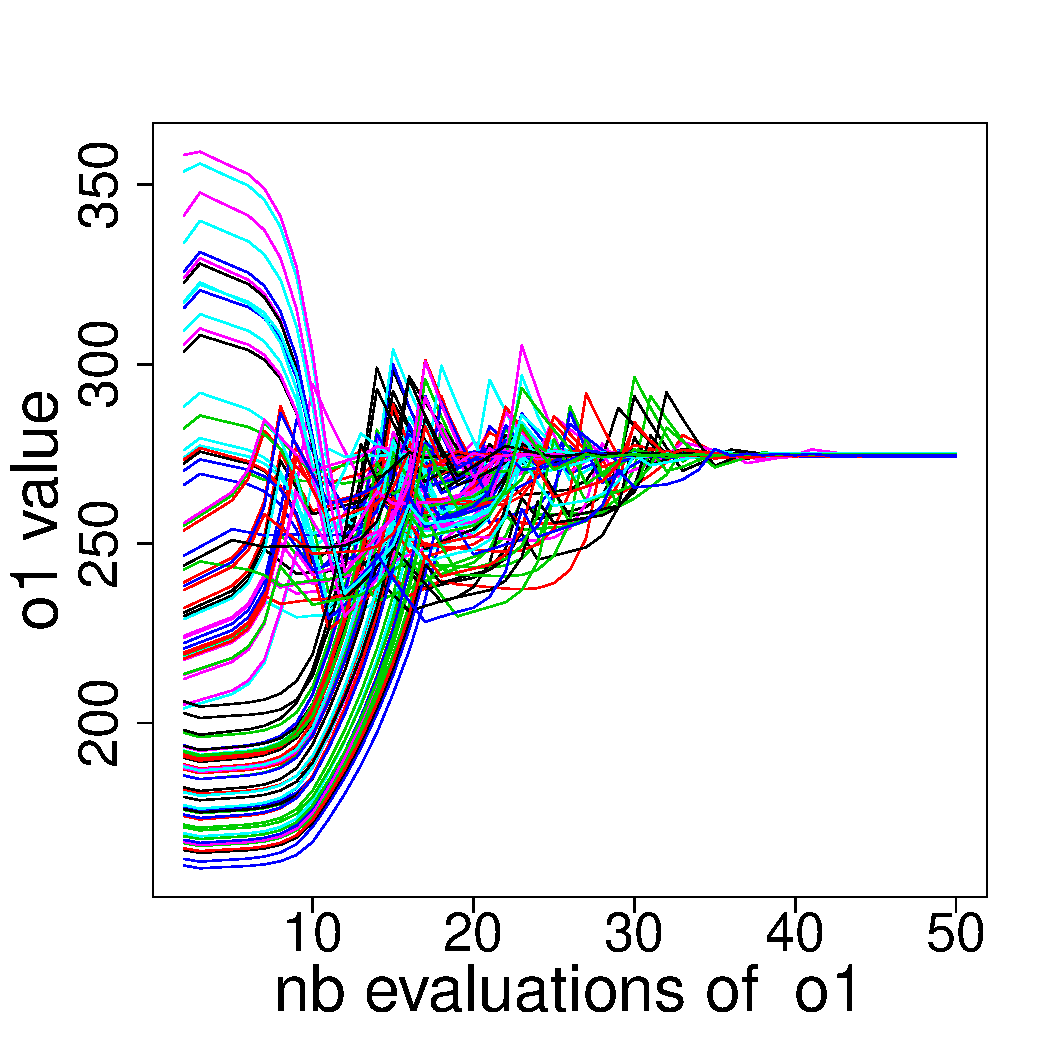
\includegraphics[width = \textwidth]{./R_figs/generated/o1}	
	\end{subfigure}
	\hfill%for spacing
	\begin{subfigure}[b]{0.4\textwidth}
		\centering
		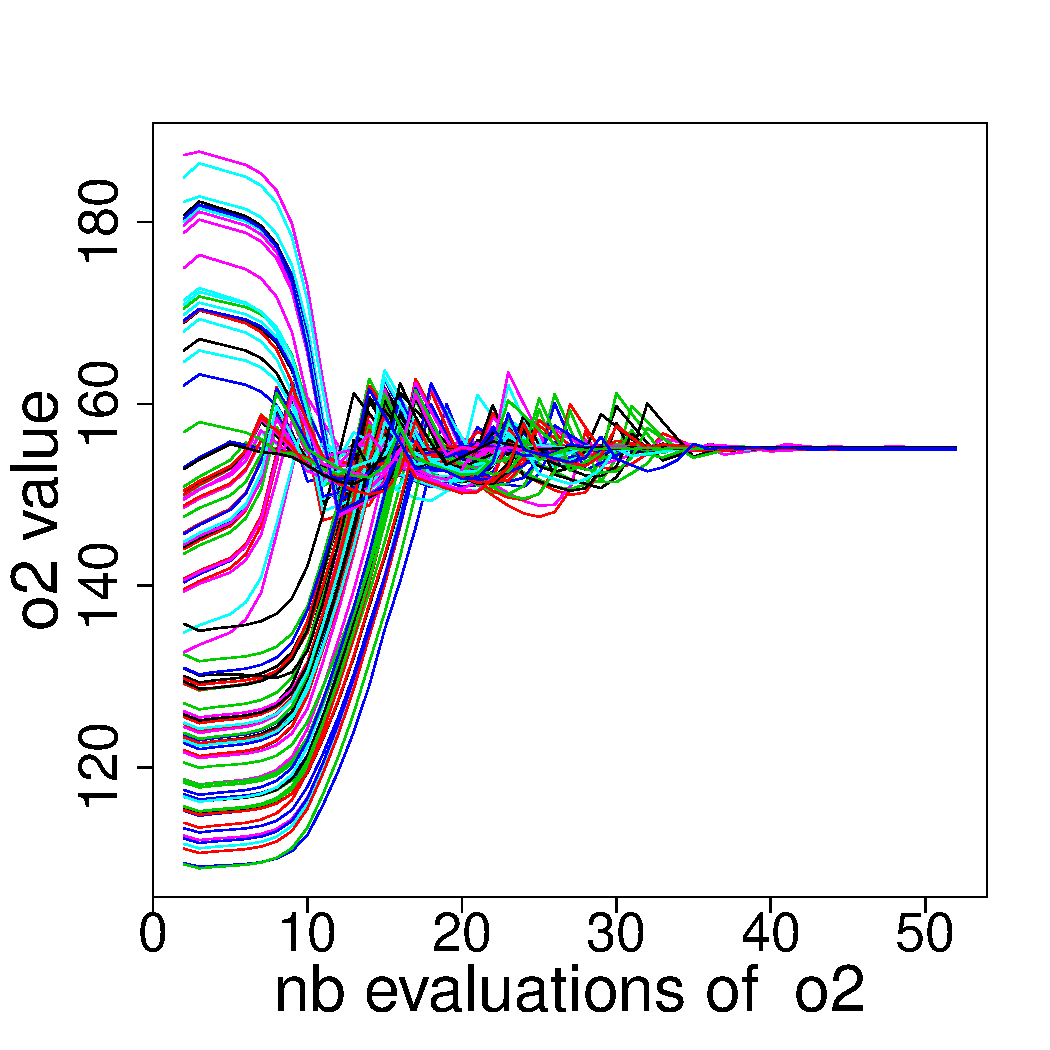
\includegraphics[width = \textwidth]{./R_figs/generated/o2}	
	\end{subfigure}
	\caption{Convergence of the Turbofan objectives for 100 random starting points}
	\label{snecma_res}
\end{figure}

\section{Viennet1}

The Viennet1 test case is part of a series of problems proposed in \cite{viennet1996multicriteria} to evaluate multi-criteria optimization techniques. This problem involves three objectives. Its analytical formulation is:
\begin{align*}
\text{Minimize } 	&o1 = x^2 + (y-1)^2 \\
								&o2 = x^2 + (y+1)^2 \\
								&o3 = (x-1)^2 + y^2 +2\\
\text{where } 		&x, y \in  [-4;4]						
\end{align*}				

\figurename{} \ref{viennet_res} illustrates the convergence of the system toward a valid solution with 100 executions from randomly chosen starting points, using only internal optimization mechanisms.

\begin{figure}[h]

	\begin{subfigure}[b]{0.32\textwidth}
		\centering
		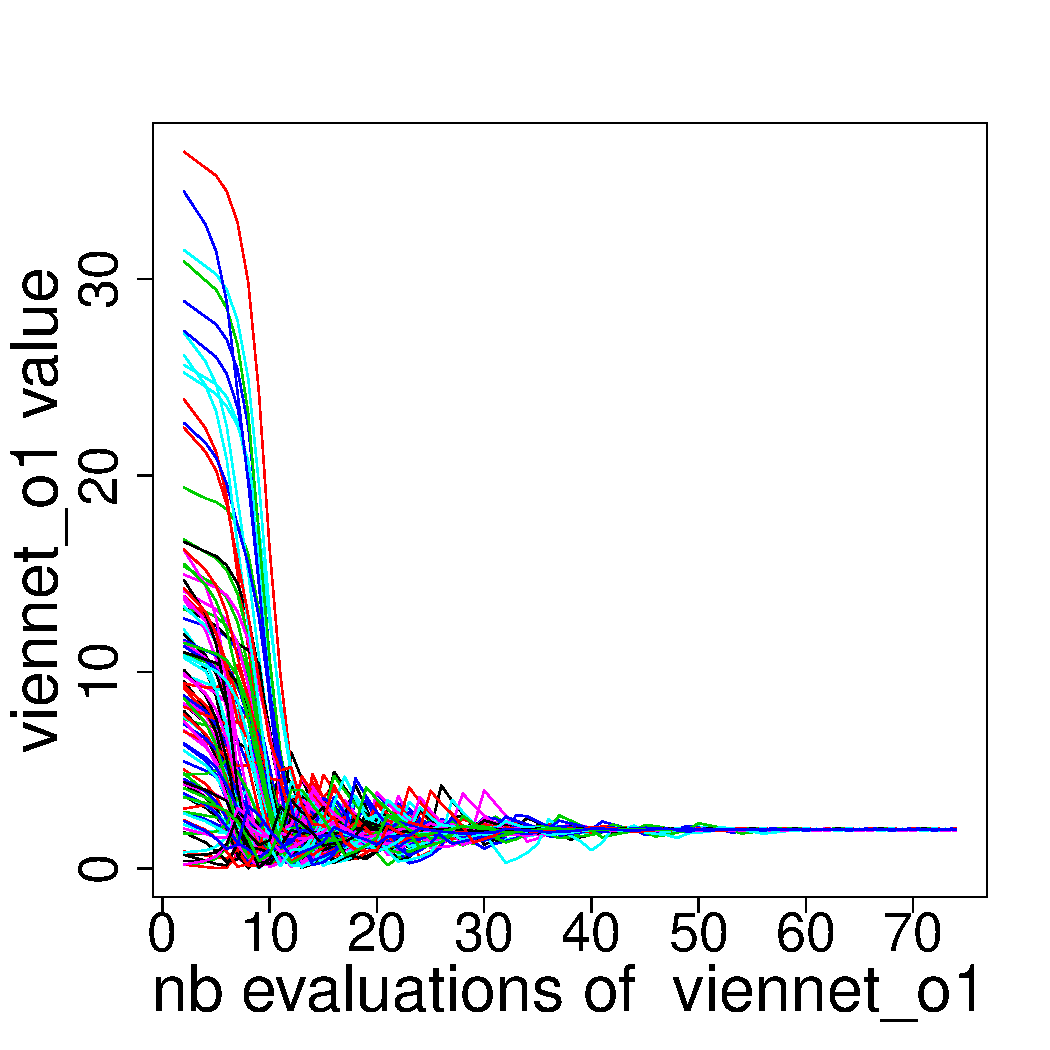
\includegraphics[width = \textwidth]{./R_figs/generated/viennet_o1}	
	\end{subfigure}
	\hfill%for spacing
	\begin{subfigure}[b]{0.32\textwidth}
		\centering
		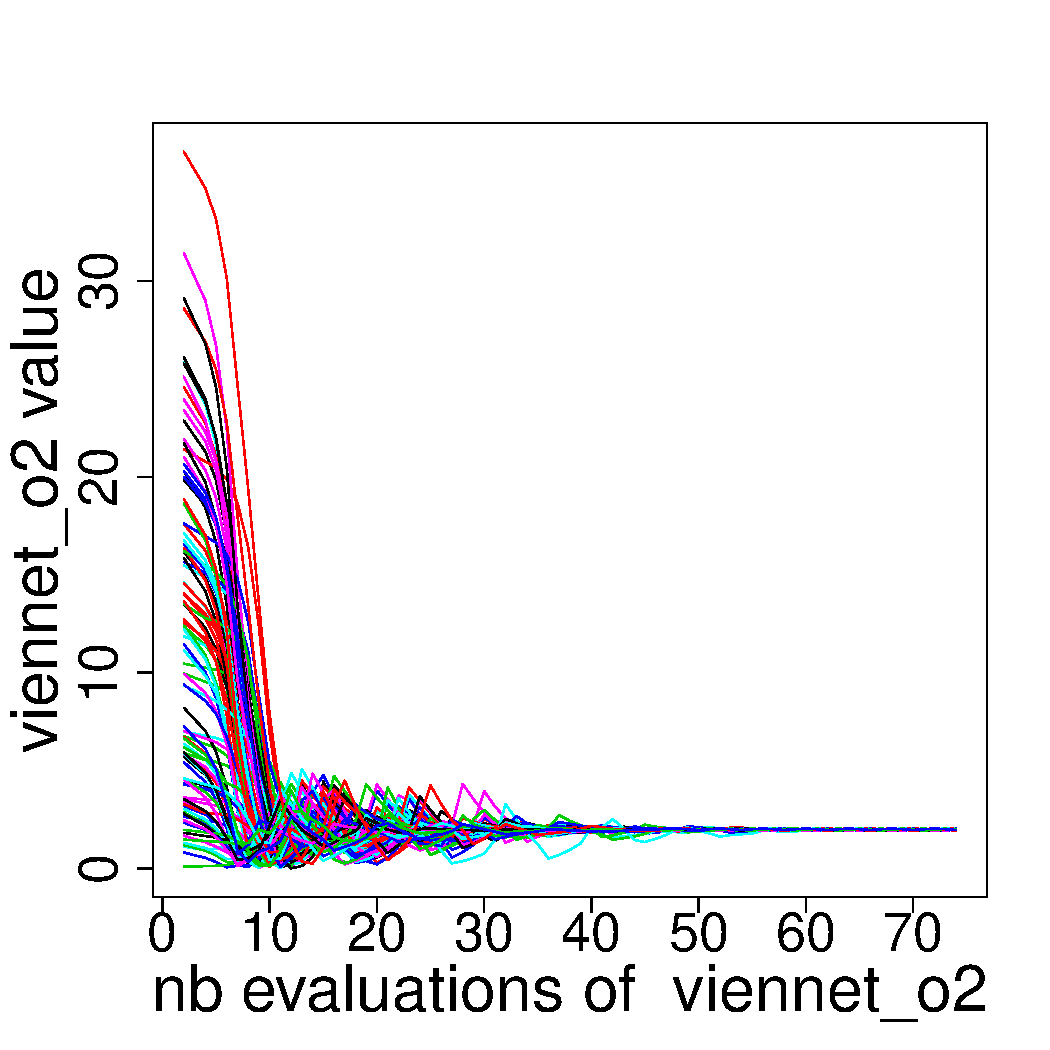
\includegraphics[width = \textwidth]{./R_figs/generated/viennet_o2}	
	\end{subfigure}
	\hfill%for spacing
	\begin{subfigure}[b]{0.32\textwidth}
		\centering
		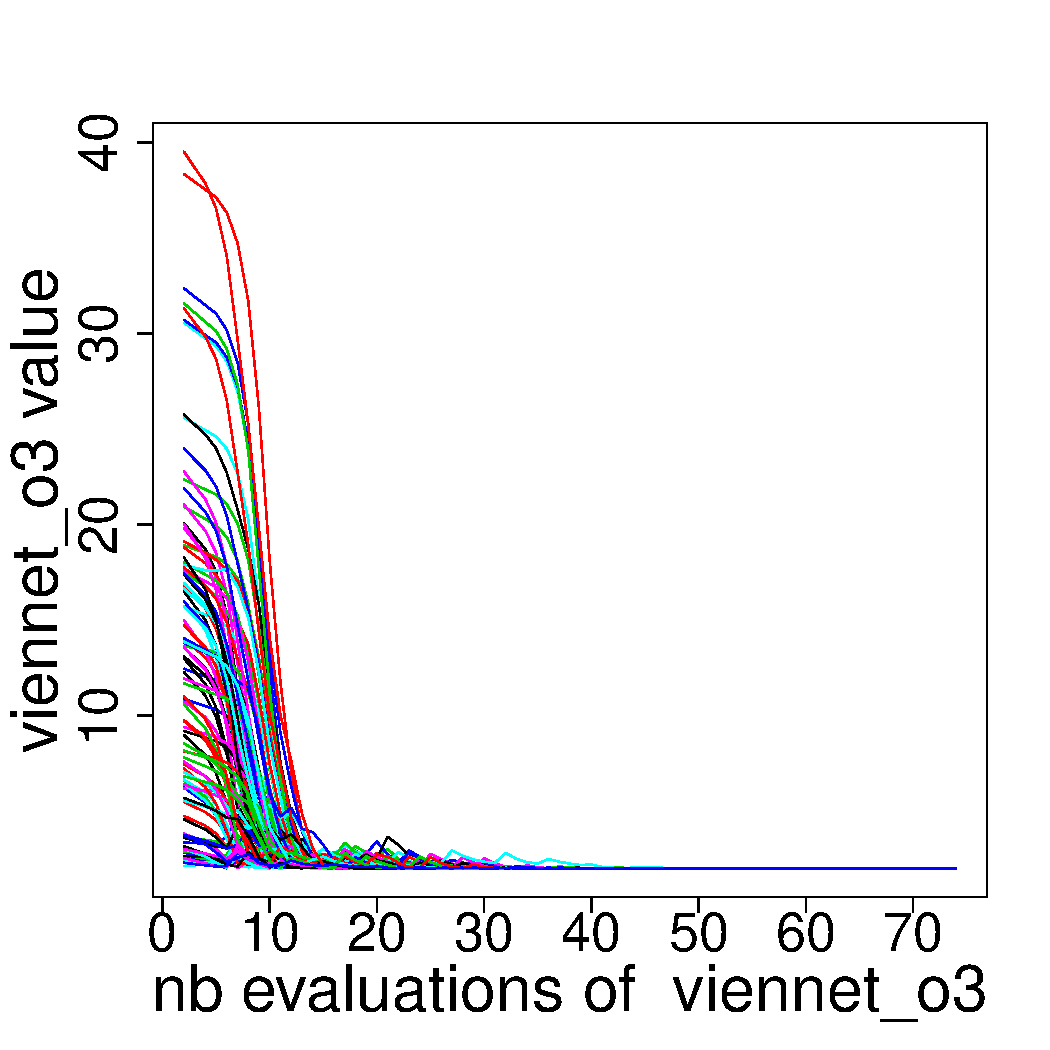
\includegraphics[width = \textwidth]{./R_figs/generated/viennet_o3}	
	\end{subfigure}
	\caption{Convergence of Viennet1 objectives for 100 random starting points}
	\label{viennet_res}
\end{figure}

\section{Rosenbrock's valley}

Rosenbrock's valley is non-convex function commonly used to test convergence capabilities of an optimization method \cite{Rosenbrock01011960}.

The analytical formulation of this problem (for two dimensions) is 
$$\text{Minimize } f(x,y) = (1-x)^2 + 100(y - x^2)^2$$

The Rosenbrock's valley problem is interesting in the fact that the global minimum is \enquote{hidden} into a narrow parabolic valley. The optimization method must thus get down into the valley and manage to follow its bottom until reaching the global optimum. Consequently it is a very adequate problem to test the cooperative trajectories mechanisms of our system.

The results presented on \figurename{} \ref{rosenbrock_res} are for the two-dimensional version of the problem with a definition domain of [-5; 5] for each \emph{design variable}.

\begin{figure}
\centering
	\begin{subfigure}[b]{0.45\textwidth}
		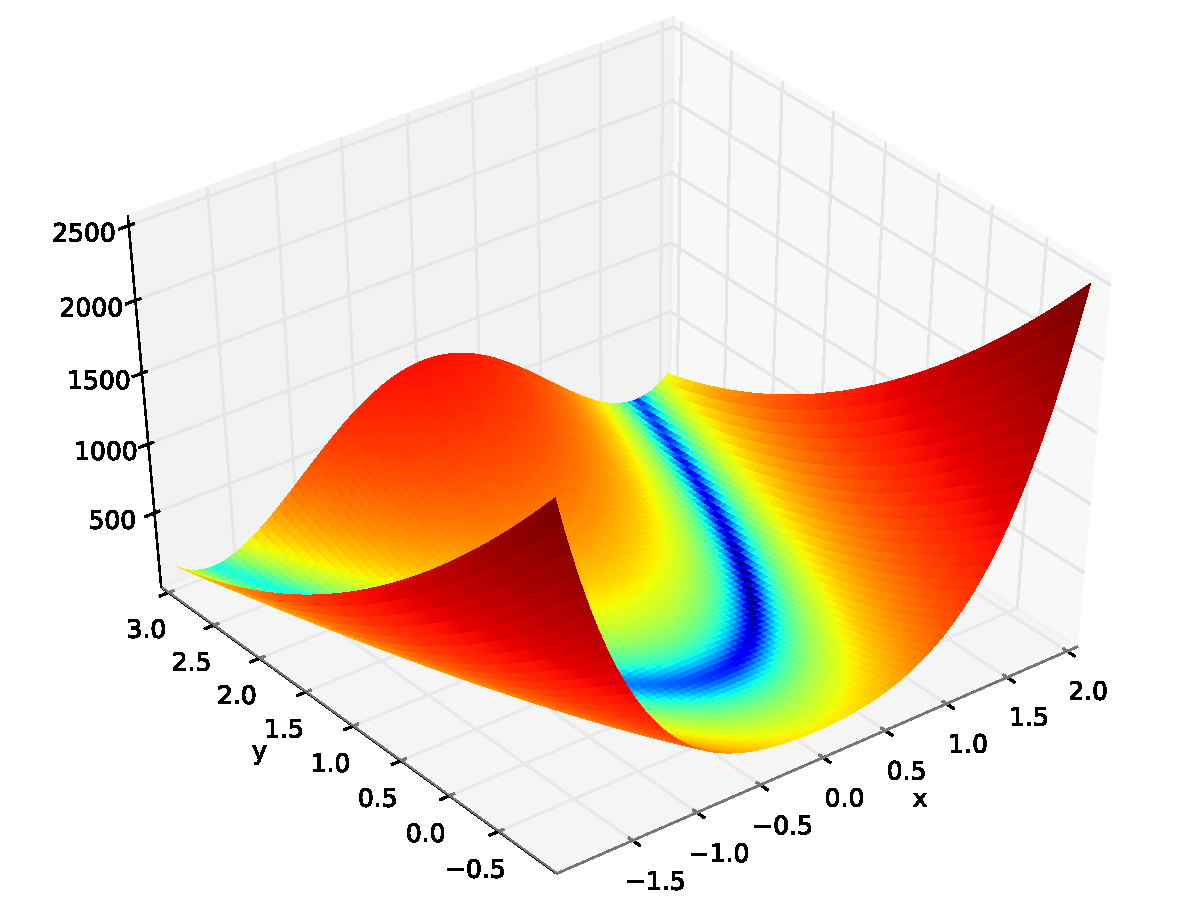
\includegraphics[width=\textwidth]{Rosenbrock_function}
		\caption{Rosenbrock's valley (from \href{http://commons.wikimedia.org/wiki/File:Rosenbrock_function.svg}{Martin Doege})}\label{rosenbrock_plot}
	\end{subfigure}
	%
	\hfill%for spacing
	%
	\begin{subfigure}[b]{0.45\textwidth}	
		\centering
		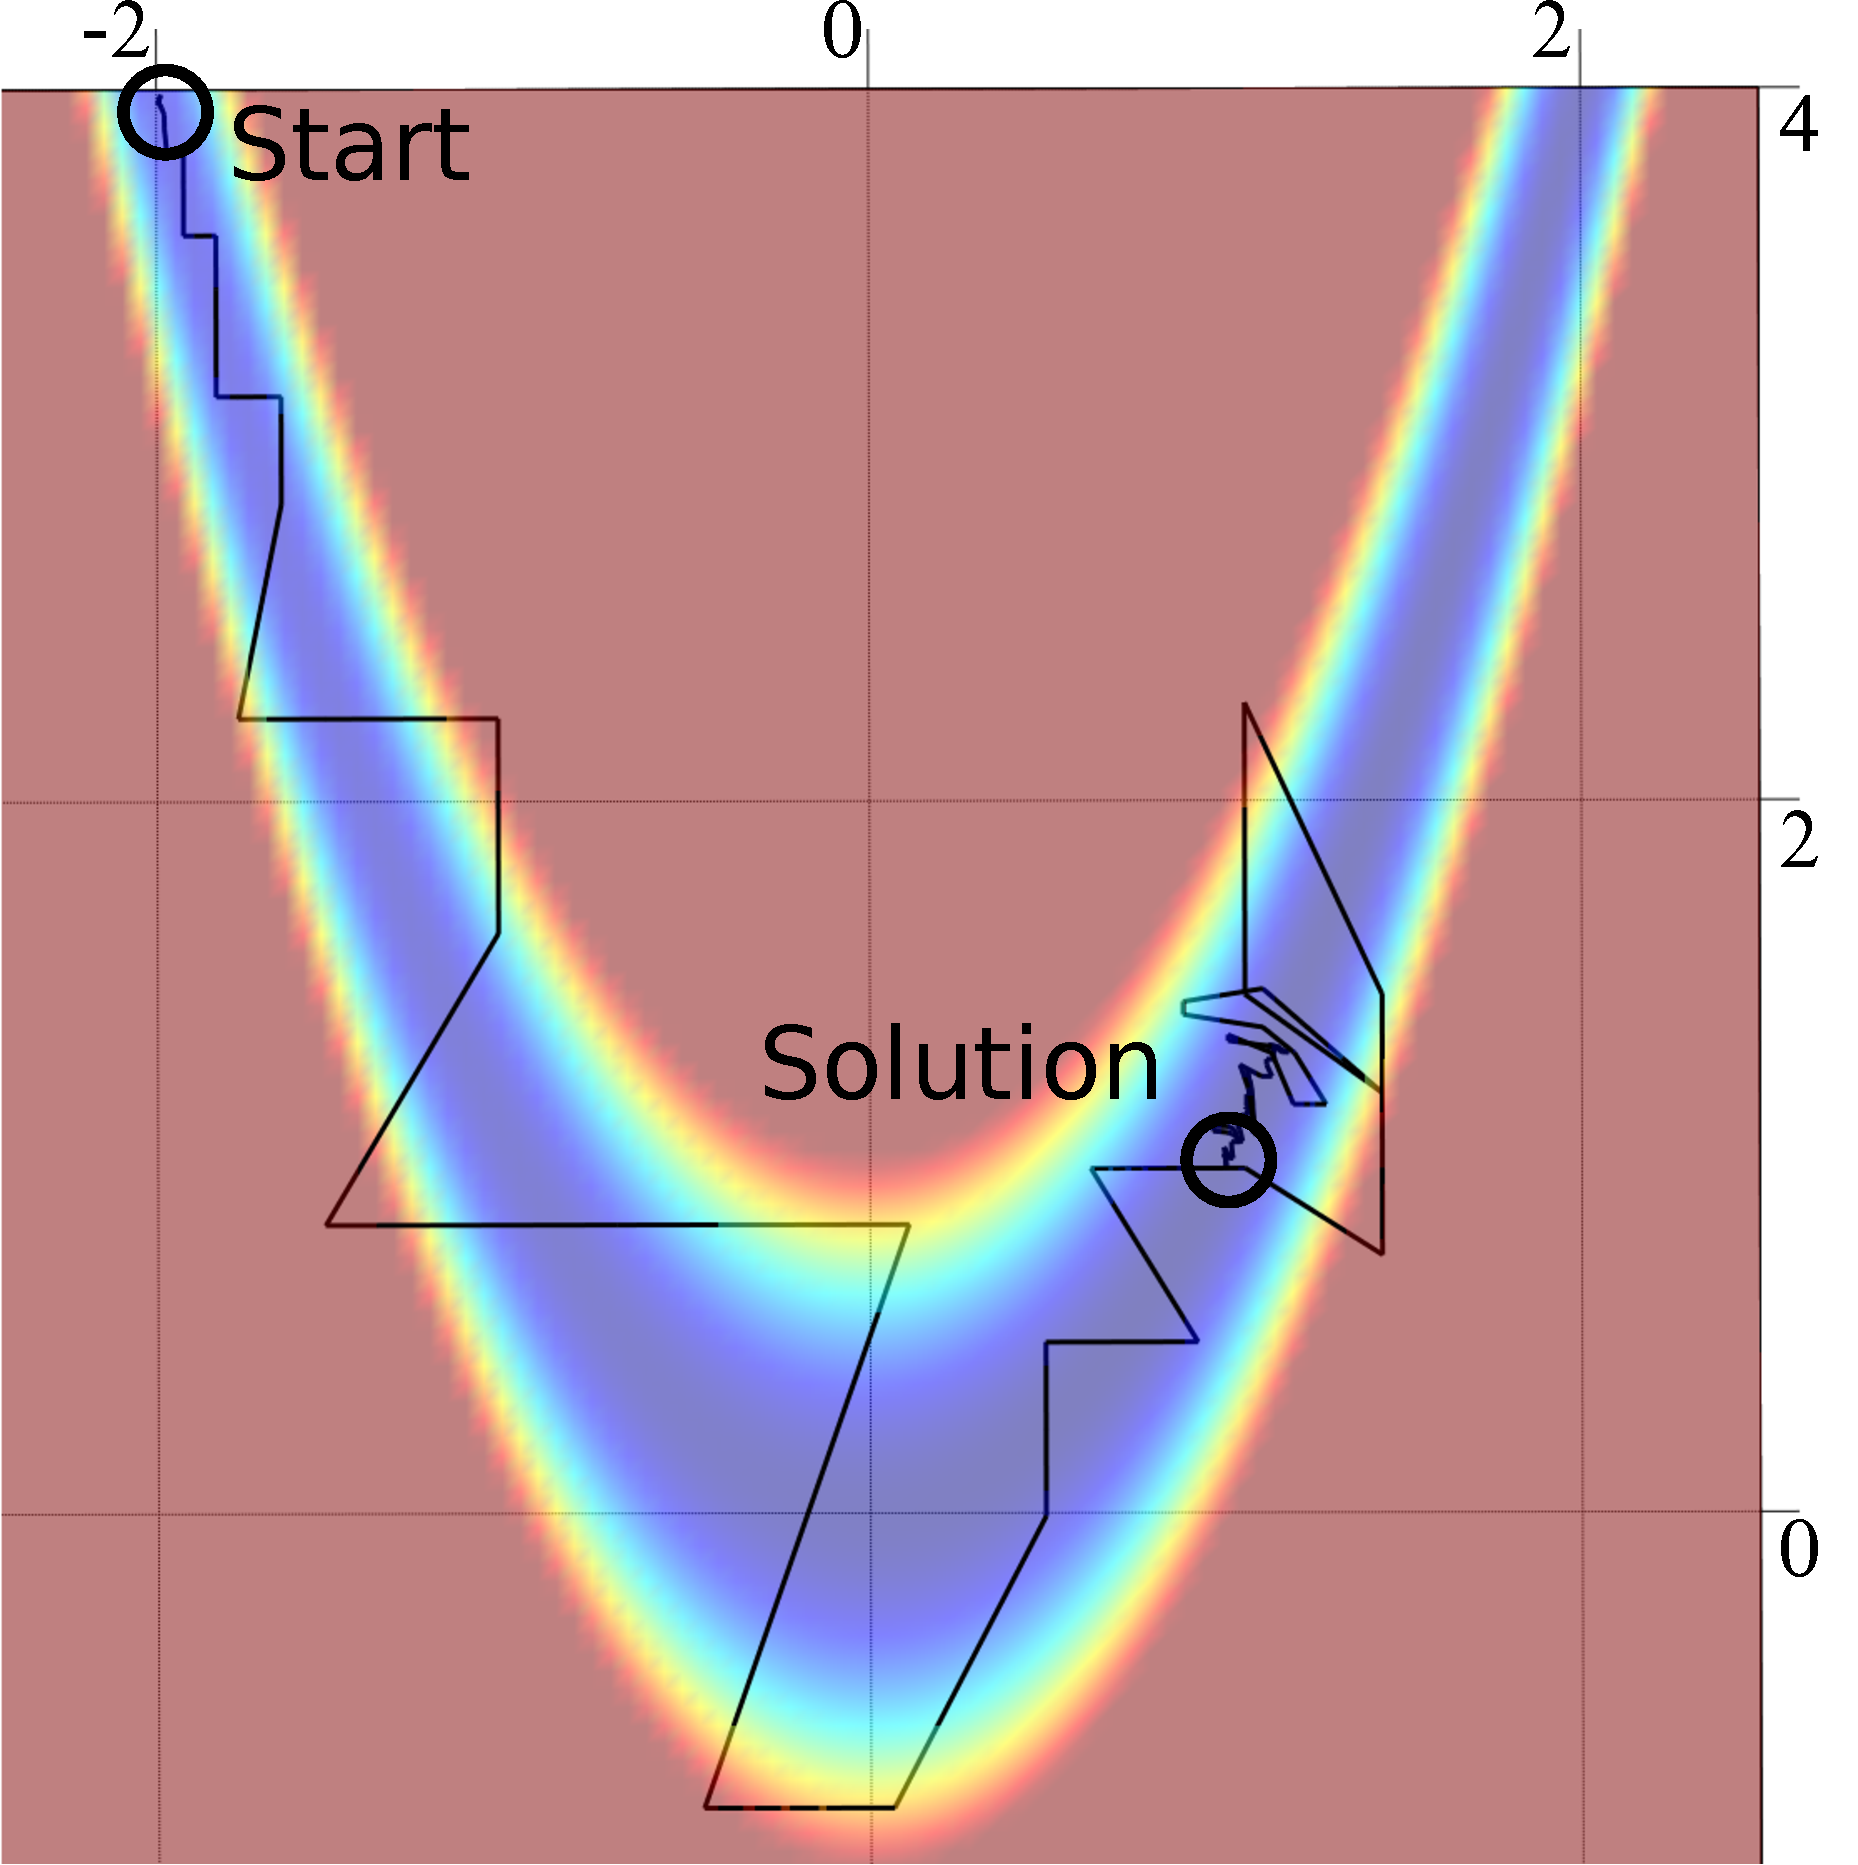
\includegraphics[width=\textwidth]{cooperative_trajectories_example}
		\caption{Example of cooperative trajectories on Rosebrock's valley (starting point (-2, 4))}\label{collective_traj_rosenbrock_plot}
	\end{subfigure}
	
	\begin{subfigure}{0.4\textwidth}
		\centering
    	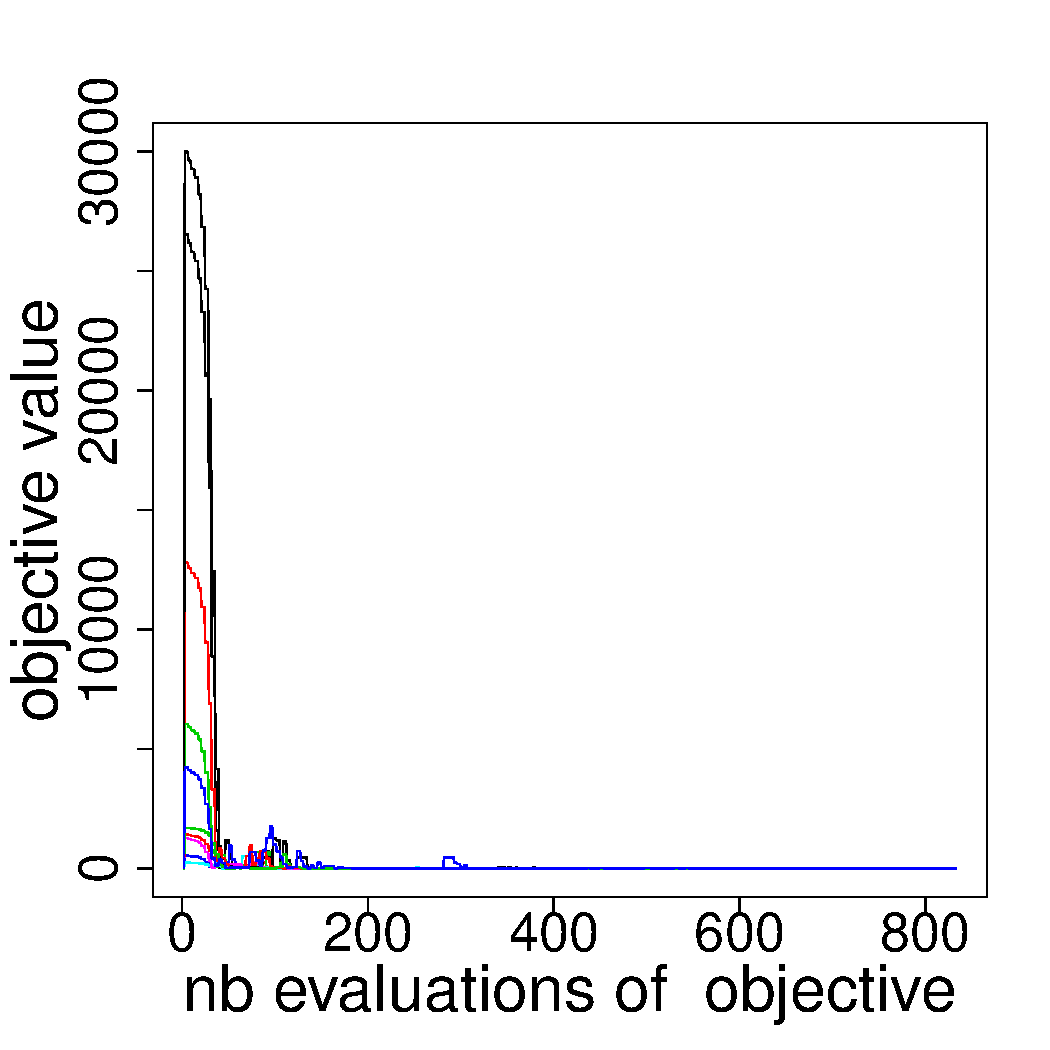
\includegraphics[width = \textwidth]{./R_figs/generated/objective}	
		\caption{Convergence of Rosenbrock objective for 100 random starting points}\label{rosenbrock_res}
	\end{subfigure}
\end{figure}

This problem was also used in \cite{Ilan:1994:MOM:887207} as an application example of the Collaborative Optimization method, presented in chapter \ref{MDO_chapter} (with performances varying from 141 to 1556  total iterations depending on the additional information used).

\section{Alexandrov Problem}

Our last test case is inspired from an academic example taken in literature by Alexandrov and al\cite{alexandrov2002analytical}. This example presents many of the commons characteristics of MDO problems: a cycle (albeit converging) and multiple criteria requiring cooperative trajectories. In the original article, the example was used to illustrate some properties of Collaborative Optimization, which we presented earlier, in terms of reformulation. While the paper only gave the structure of the problem, we adapted it with meaningful values and equations.

The mathematical formulation of the problem and the corresponding agent graph can be seen in \figurename{} \ref{alexandrov}. Interestingly, the NDMO representation is quite similar to the one adopted by the original authors of the problem.

\begin{figure}
\centering
	\begin{subfigure}[b]{0.4\textwidth}
		$\begin{array}{c}
			a_1 = (l_1 - a_2)/2 \\
			a_2 = (l_2 - a_1)/2 \\
			min \; \frac{1}{2}(a_1^2 + 10a_2^2 + 5(s-3)^2) \\
			subject \; to \\
			s + l_1 \leq 1 \\
			-s + l_2 \leq -2
		\end{array}$
		\caption{mathematical formulation.}\label{alexandrov:math}
	\end{subfigure}
	\hfill%for spacing
	\begin{subfigure}[b]{0.4\textwidth}
		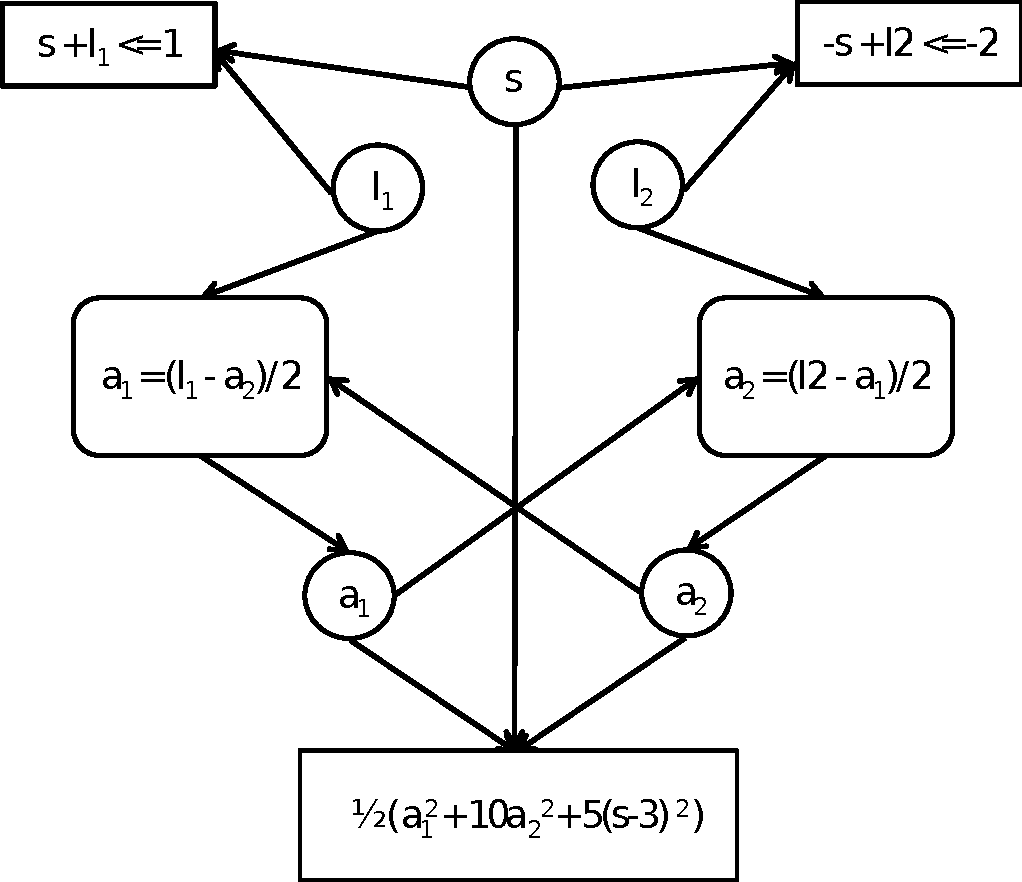
\includegraphics[width=\textwidth]{testcases-Alexandrov}%screen_Alexandrov}%}
		\caption{corresponding agent graph.}\label{alexandrov:graph}
	\end{subfigure}
\caption{Alexandrov problem}\label{alexandrov}
%\vspace{-20pt}
\end{figure}

On \figurename{} \ref{alexandrov_res_one}, the behavior of the \emph{design variables} agents l1, l2 and s, as well the evolution of the objective, can be observed on one instance of the problem with random starting points.

\begin{figure}
\centering
  	\begin{subfigure}[b]{0.4\textwidth}
		\centering
		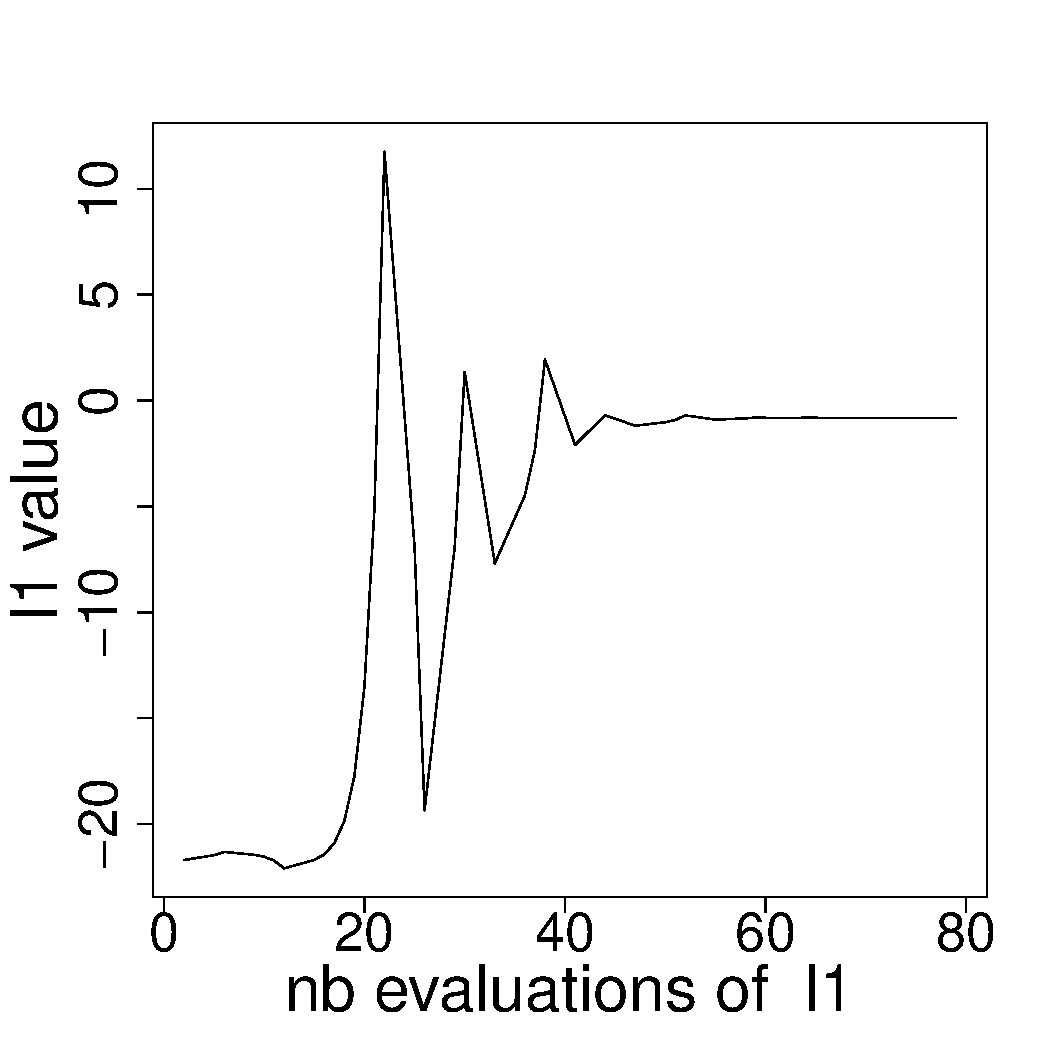
\includegraphics[width=\textwidth]{./R_figs/generated/l1_one_run}
		%\vspace{-20pt}
		\label{alexandrov_res_one:l1}
	\end{subfigure}
	\begin{subfigure}[b]{0.4\textwidth}
		\centering
		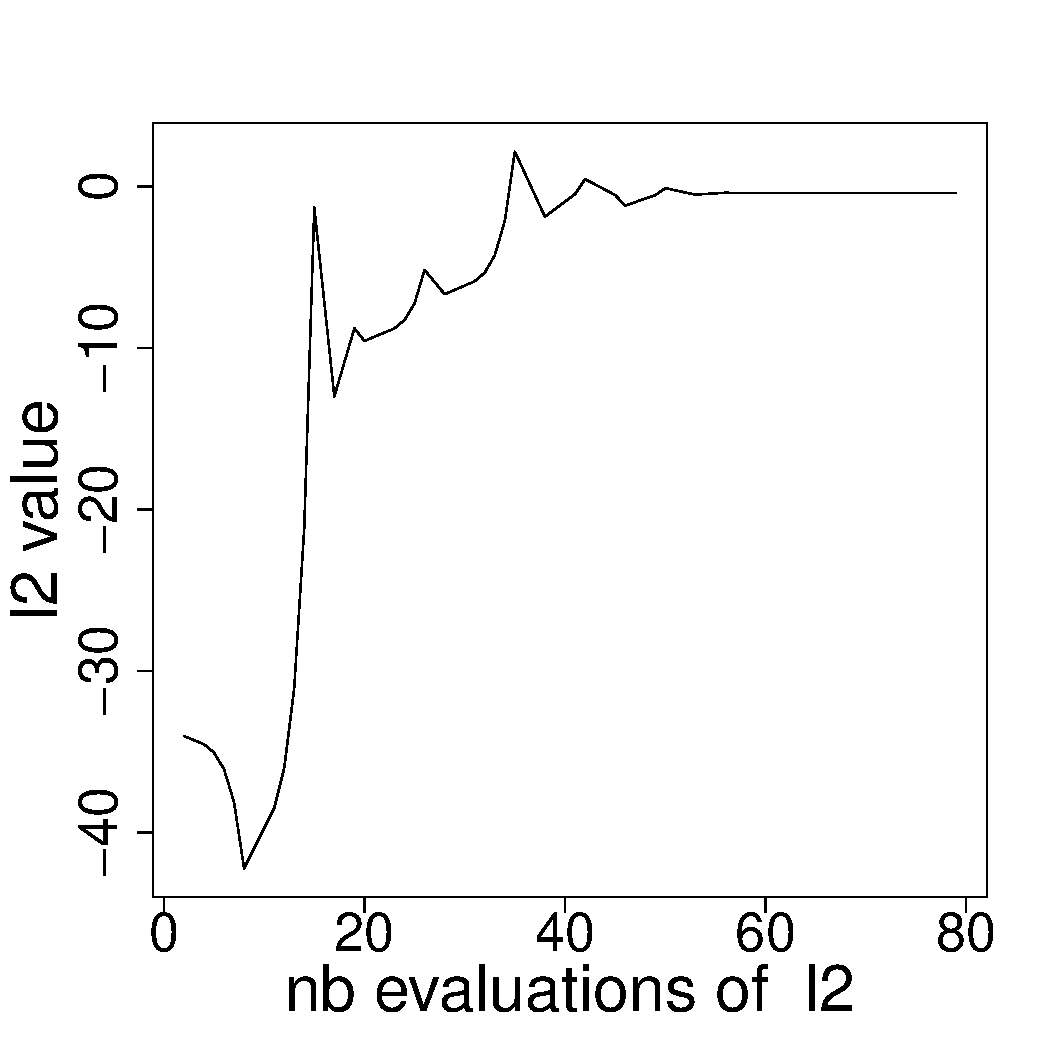
\includegraphics[width=\textwidth]{./R_figs/generated/l2_one_run}
		%\vspace{-20pt}
		\label{alexandrov_res_one:l2}
	\end{subfigure}
	\vspace{-20pt}
	\\
	\begin{subfigure}[b]{0.4\textwidth}
		\centering
		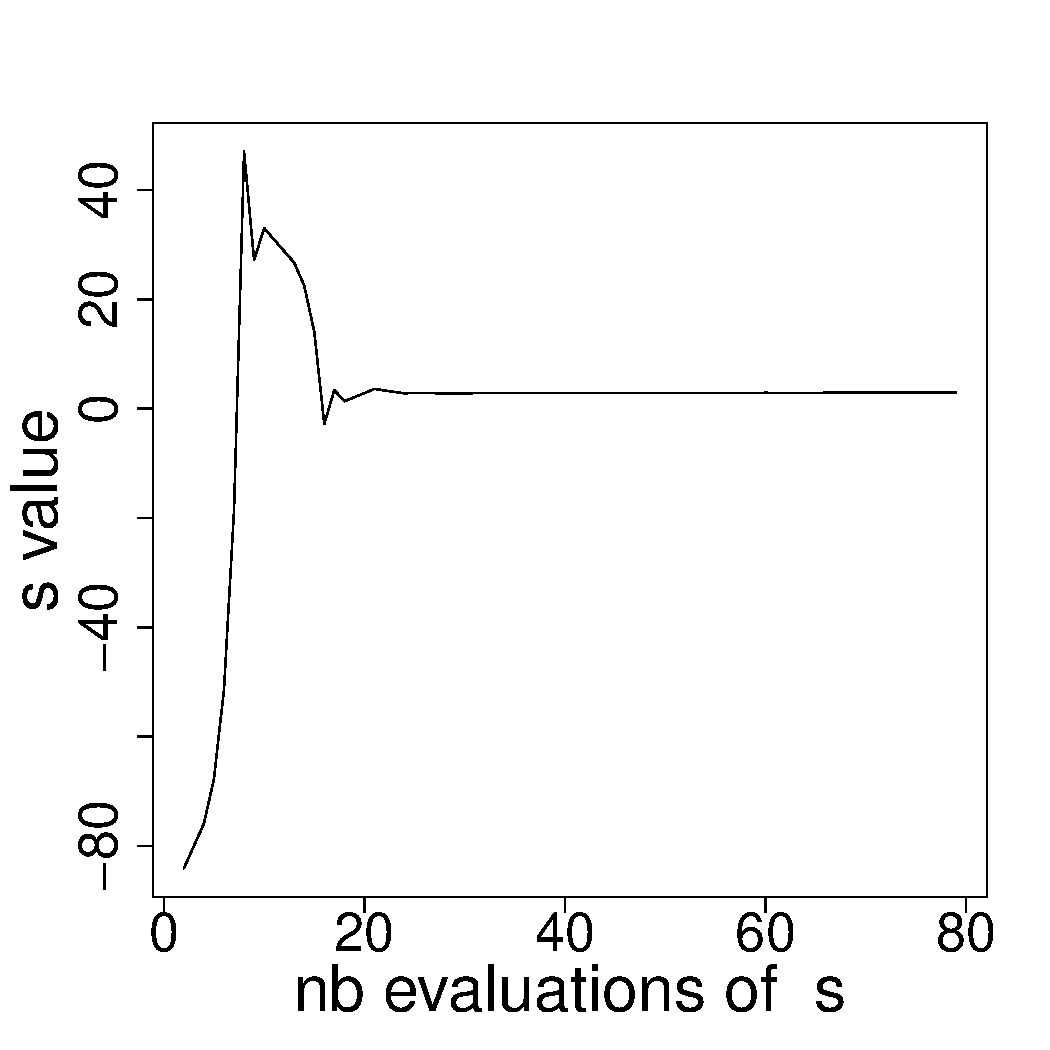
\includegraphics[width=\textwidth]{./R_figs/generated/s_one_run}
		%\vspace{-20pt}
		\label{alexandrov_res_one:s}
	\end{subfigure}
	\begin{subfigure}[b]{0.4\textwidth}
		\centering
		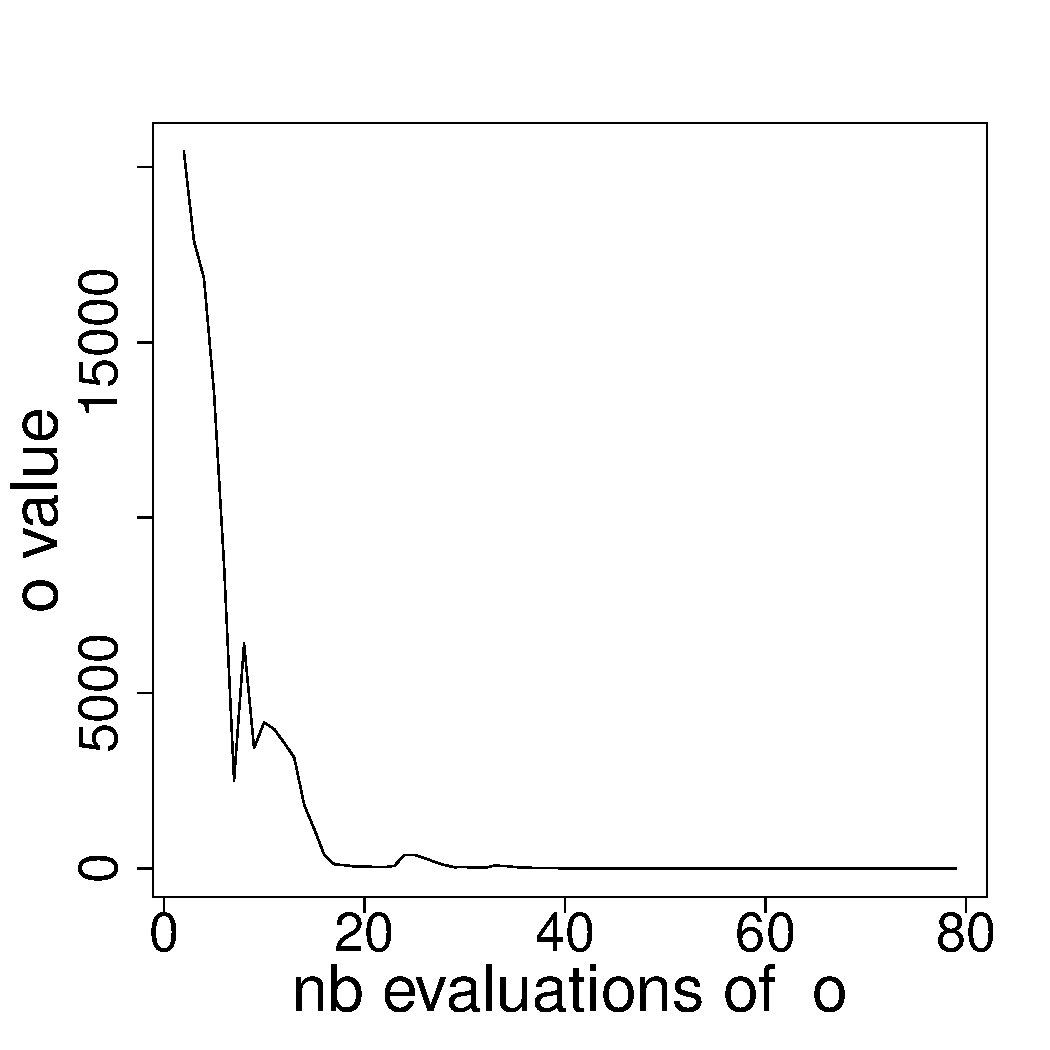
\includegraphics[width=\textwidth]{./R_figs/generated/o_one_run}
		%\vspace{-20pt}
		\label{alexandrov_res_one:o}
	\end{subfigure}
	
	\caption{Alexandrov agents behavior}
	\label{alexandrov_res_one}

\end{figure}

On \figurename{} \ref{alexandrov_res}, we show the evolution of the objective over 100 iterations with  starting points  for each \emph{design variable} randomly drawn over the interval [-100; 100]. We can see how the system converges towards the same optimum despite the wildly different initial conditions.

\begin{figure}
\centering
    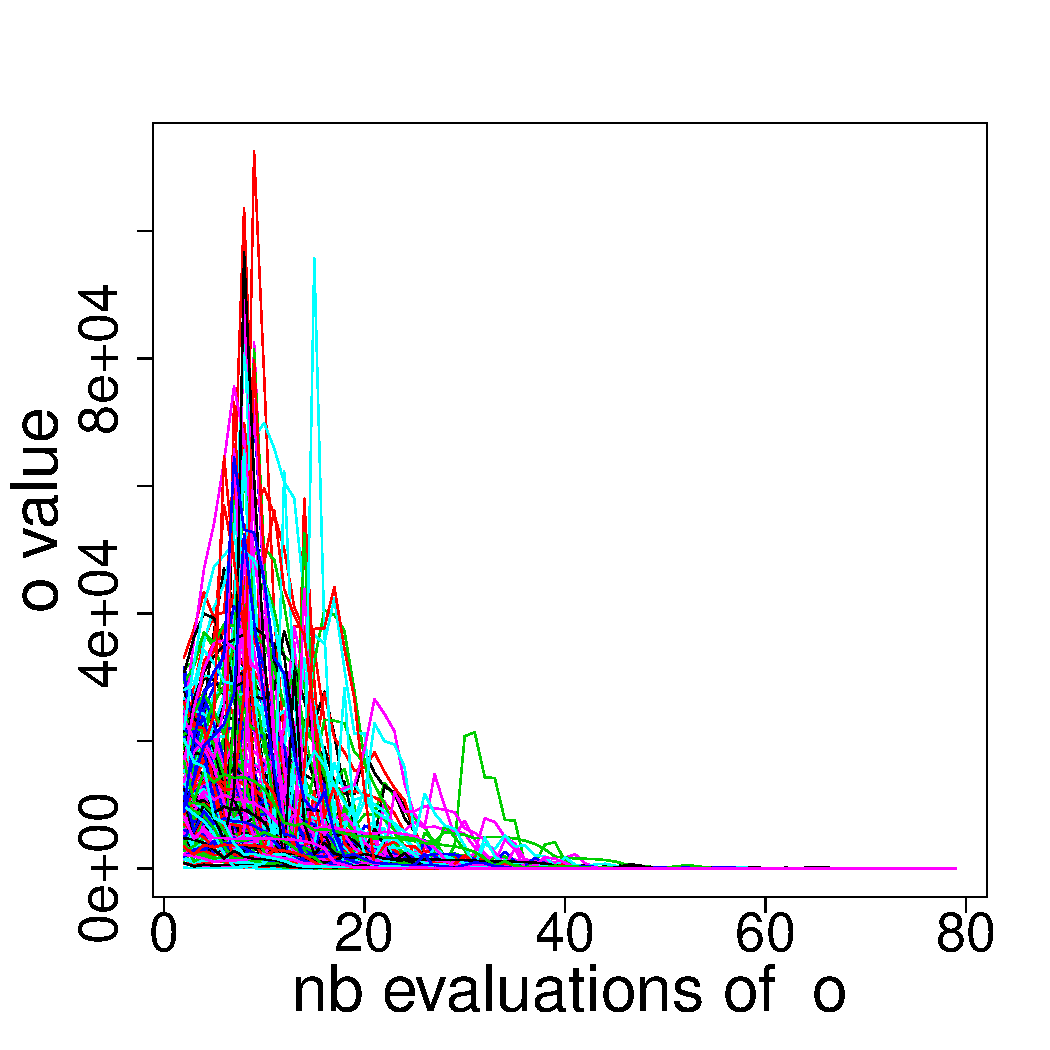
\includegraphics[width=0.4\textwidth]{./R_figs/generated/o}
	\caption{Convergence of the Alexandrov objective for 100 random starting points}
	\label{alexandrov_res}
\end{figure}

\section{Analysis of Academic Test Cases}

In this section we presented several academic test cases exhibiting classical properties of complex continuous optimization problems. We shown how the system was able to consistently converge on each test case toward an optimum solution, for multiple starting points.

Summarized results illustrating the convergence of the system. are presented on \tablename{} \ref{experiments_res}. The first group of values represents the number of evaluations which was needed for respectively 10\%, 50\% and 90\% of the instances to find the best solution. The second group represent the average distance to the best solution (trucated at $10^{-3}$) among all instances at different times (0\% being the start 100\% being the end of the solving in the worst case).

\begin{table}
\caption{Summary of experiments results for the tests cases}\label{experiments_res}

\centering
\begin{tabular}{cccc|cccc}
	\toprule
		& \multicolumn{3}{c|}	{nb. evaluations to best}
		& \multicolumn{4}{c}	{average distance to best} \\
	\cline{2-8}
		&	10\%		& 	50\%	&		90\%	&	0\% (start)		& 	30\%	&		60\%	&	100\% (end)\\
	\toprule
	Turbofan\_o1 & 22 & 38 & 50 & 67.654 & 21.563 & 1.78 & 0.313\\
	Turbofan\_o2 & 14 & 23 & 32 & 23.876 & 2.485 & 0.387 & 0.101\\
	\midrule
	Viennet\_o1 & 8 & 17 & 29 & 8.514 & 0.458 & 0.033 & 0.021\\
	Viennet\_o2 & 9 & 15 & 27 & 9.412 & 0.37 & 0.043 & 0.021\\
	Viennet\_o3 & 9 & 14 & 23 & 10.622 & 0.102 & 0.001 & 0.0	\\
	\midrule
	Rosenbrock & 19 & 47 & 56 & 13749.427 & 123.44 & 4.564 & 2.201\\
	\midrule
	Alexandrov & 36 & 52 & 70 & 13109.169 & 1236.501 & 15.434 & 0.059\\
	\bottomrule
\end{tabular}

\end{table}

These results tend to validate the correctness of our approach, proving that the conjunction of the agents nominal behaviors and cooperative mechanisms allows to solve correct solution to diverse optimization problems.

We will now present the second part of our validation, by making experiment on larger test cases in order to validate the system behavior on complex problem and to compare the performances of our system with other complex optimization methods.

\section{Optimization under Uncertainties}

[[TODO]]

\section{Adaptation to Perturbations}

\subsection{Perturbated Alexandrov Problem}
 
On \figurename{} \ref{alexandrov_res_pert}, we can observe the reaction of the multi-agent system to a perturbation. During the solving of the previous experimentation on the problem, we changed the threshold of the constraint $s + l_1 \leq 1$ to $s + l_1 \leq -4$ (the change is indicated by a dotted line on the charts). The system dynamically adapts to the constraint changed and converges towards a new solution which satisfies the updated constraint.

\begin{figure}[]
\centering
  	\begin{subfigure}[b]{0.4\textwidth}
		\centering
		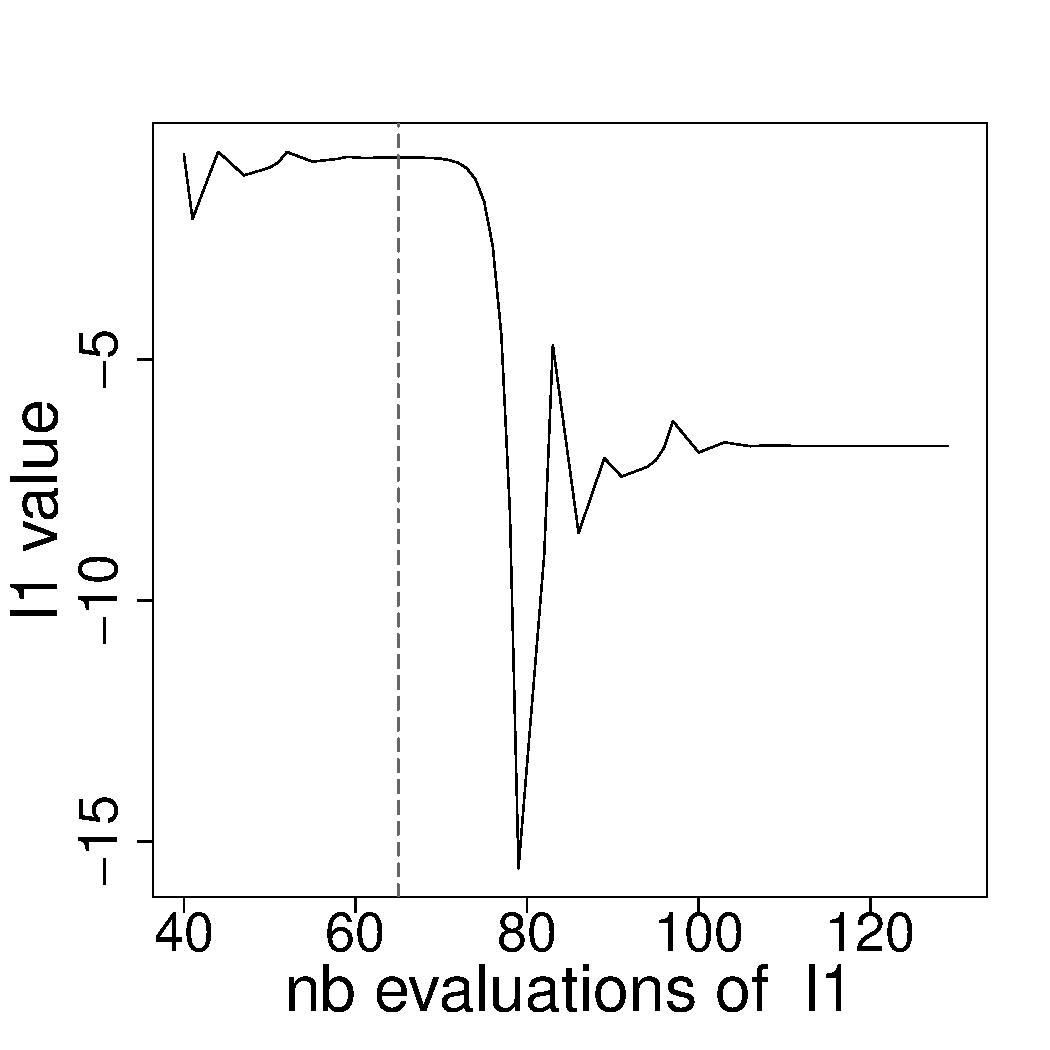
\includegraphics[width=\textwidth]{./R_figs/generated/l1_pertubated}
		\label{alexandrov_res_pert:l1}
	\end{subfigure}
	\begin{subfigure}[b]{0.4\textwidth}
		\centering
		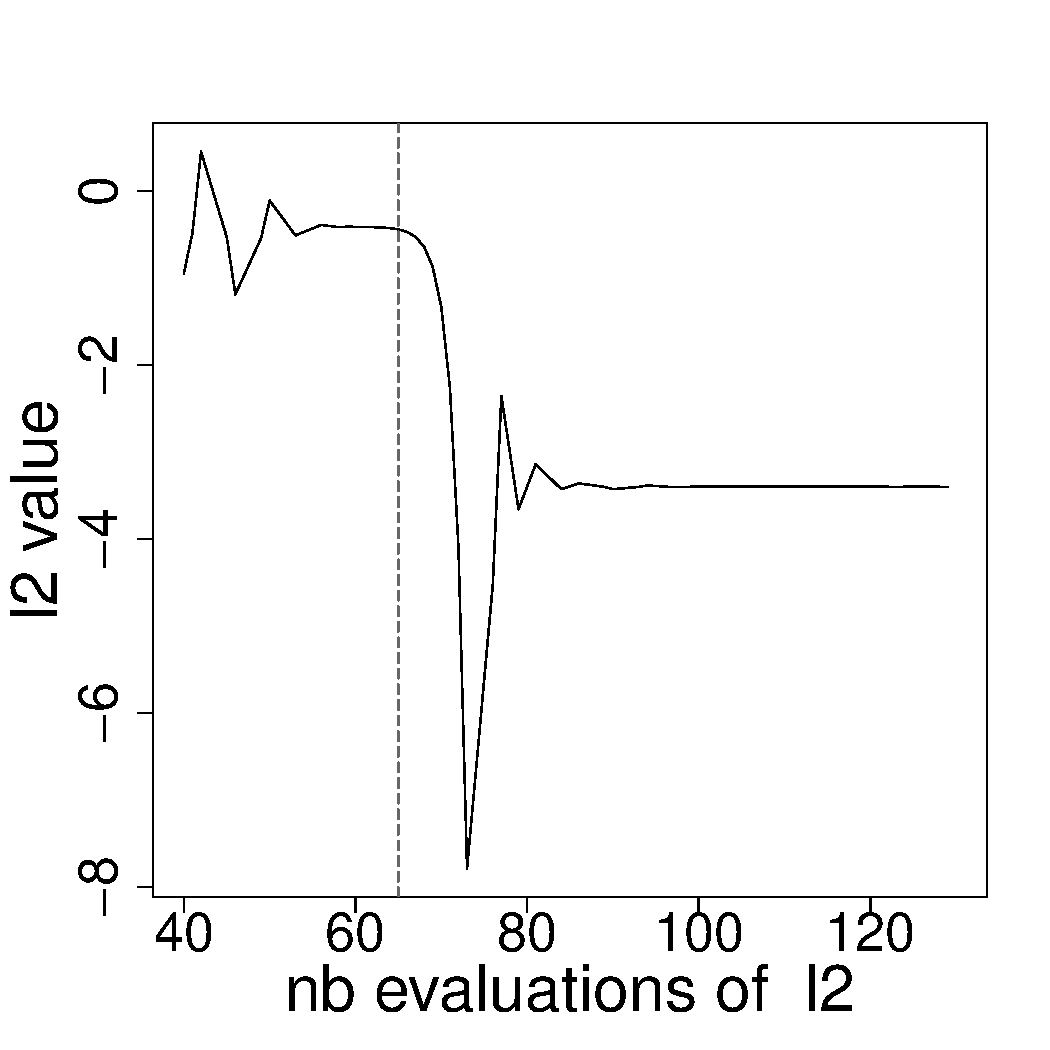
\includegraphics[width=\textwidth]{./R_figs/generated/l2_pertubated}
		\label{alexandrov_res_pert:l2}
	\end{subfigure}

	\begin{subfigure}[b]{0.4\textwidth}
		\centering
		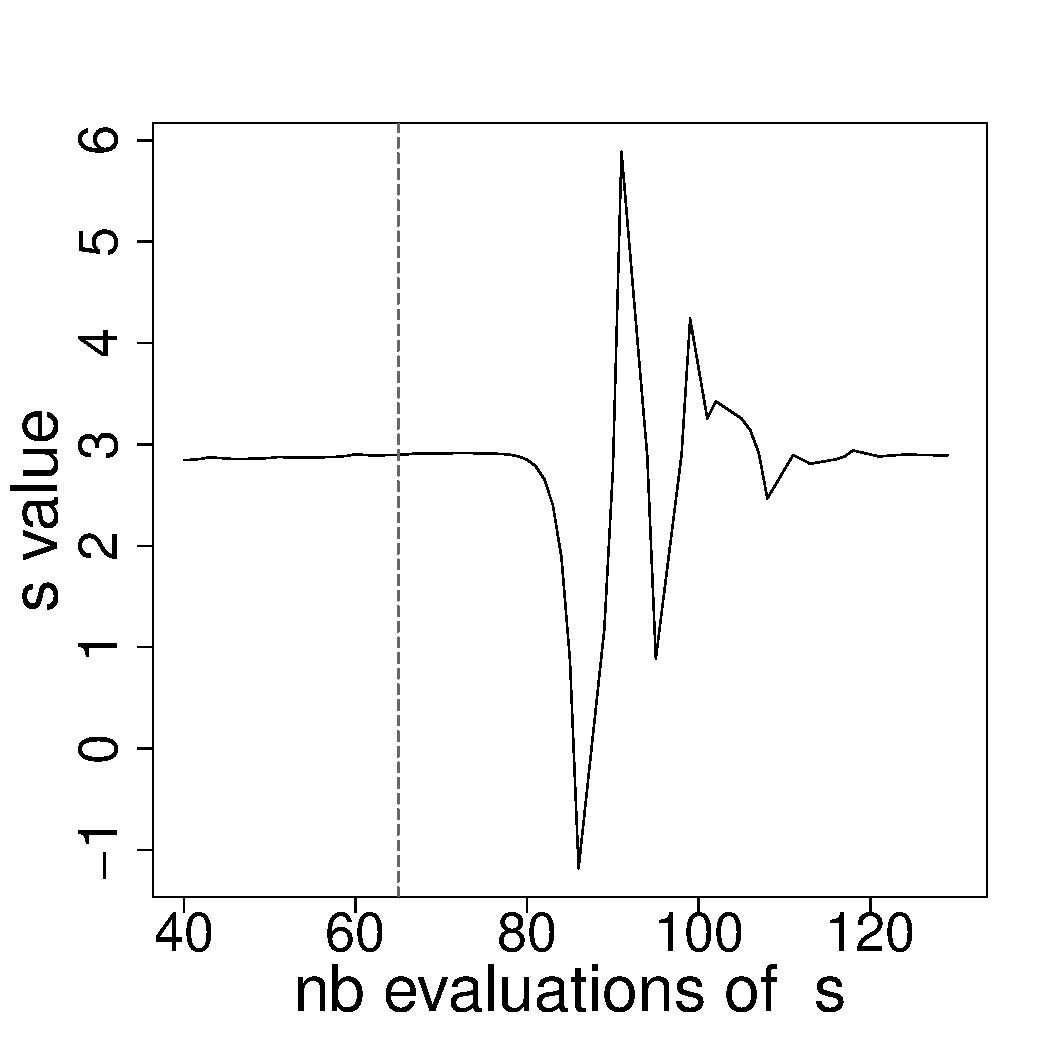
\includegraphics[width=\textwidth]{./R_figs/generated/s_pertubated}
		\label{alexandrov_res_pert:s}
	\end{subfigure}
	\begin{subfigure}[b]{0.4\textwidth}
		\centering
		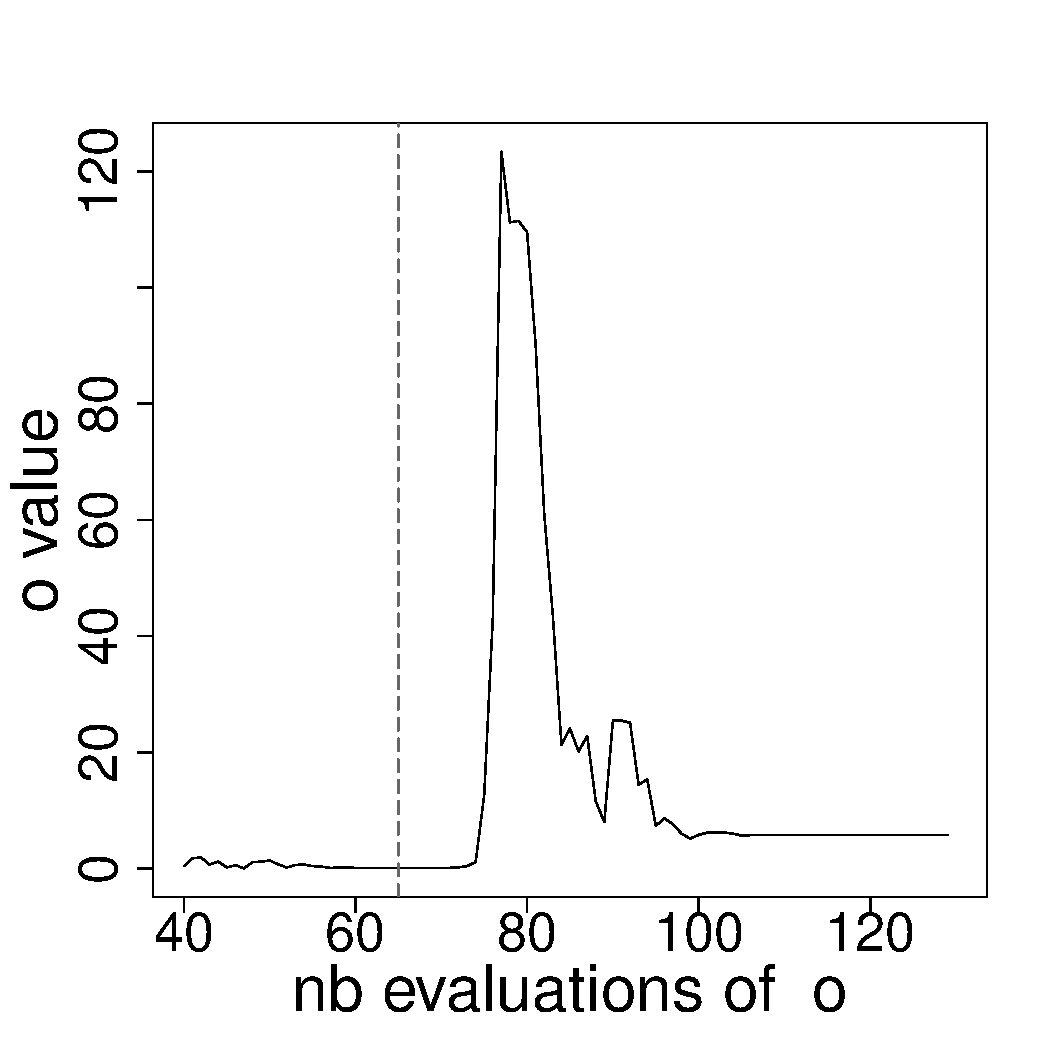
\includegraphics[width=\textwidth]{./R_figs/generated/o_pertubated}
		\label{alexandrov_res_pert:o}
	\end{subfigure}
	
	\caption{Alexandrov agents behavior with perturbation (constraint change at dotted line)}
	\label{alexandrov_res_pert}
	
\end{figure}

\subsection{Perturbated Turbofan Problem}

\begin{figure*}
\centering

  \subfloat{\begin{minipage}{0.32\textwidth}
		\centering
		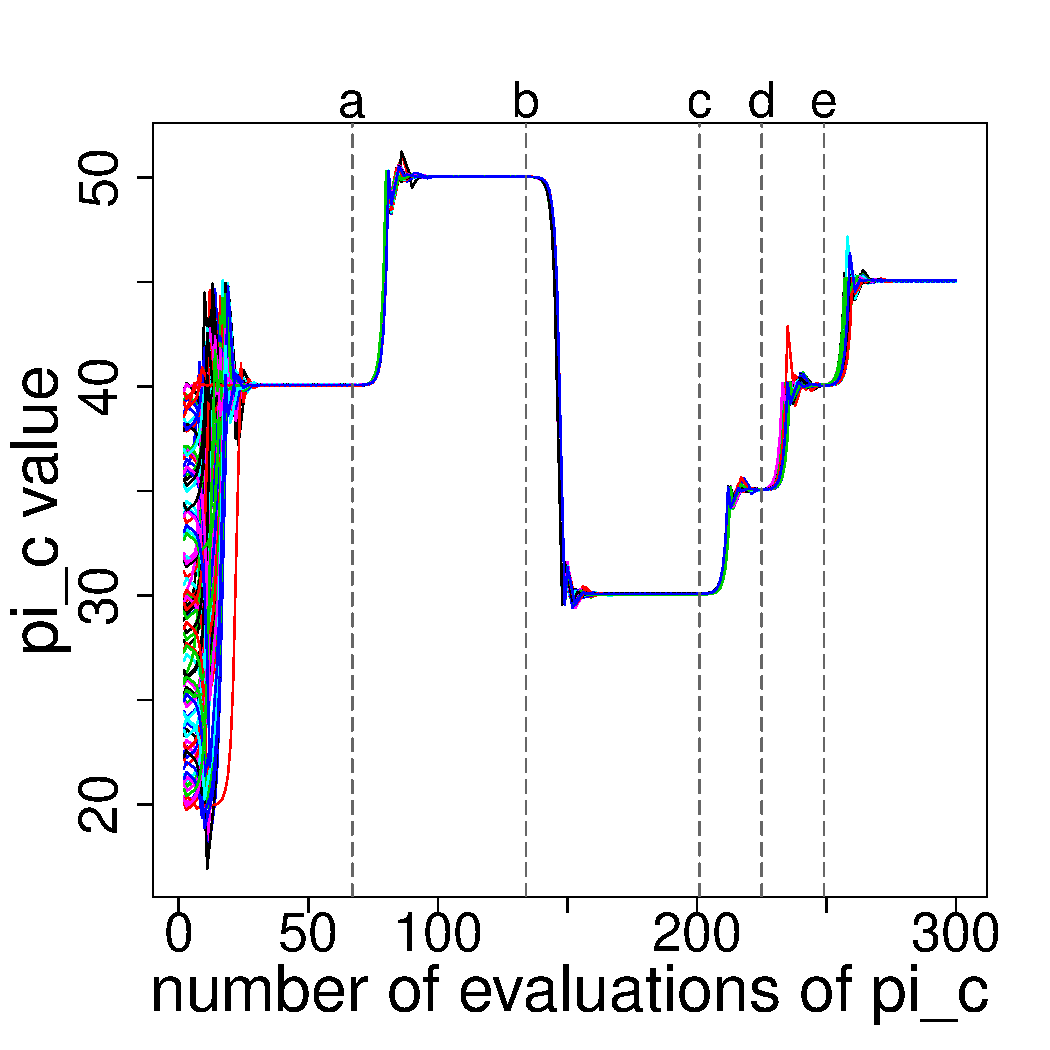
\includegraphics[width=\textwidth]{./R_figs/generated/turbofan_perturbated_pi_c}
		\label{turbofan_res_pert:pi_c}
	\end{minipage}}
	\subfloat{\begin{minipage}{0.32\textwidth}
		\centering
		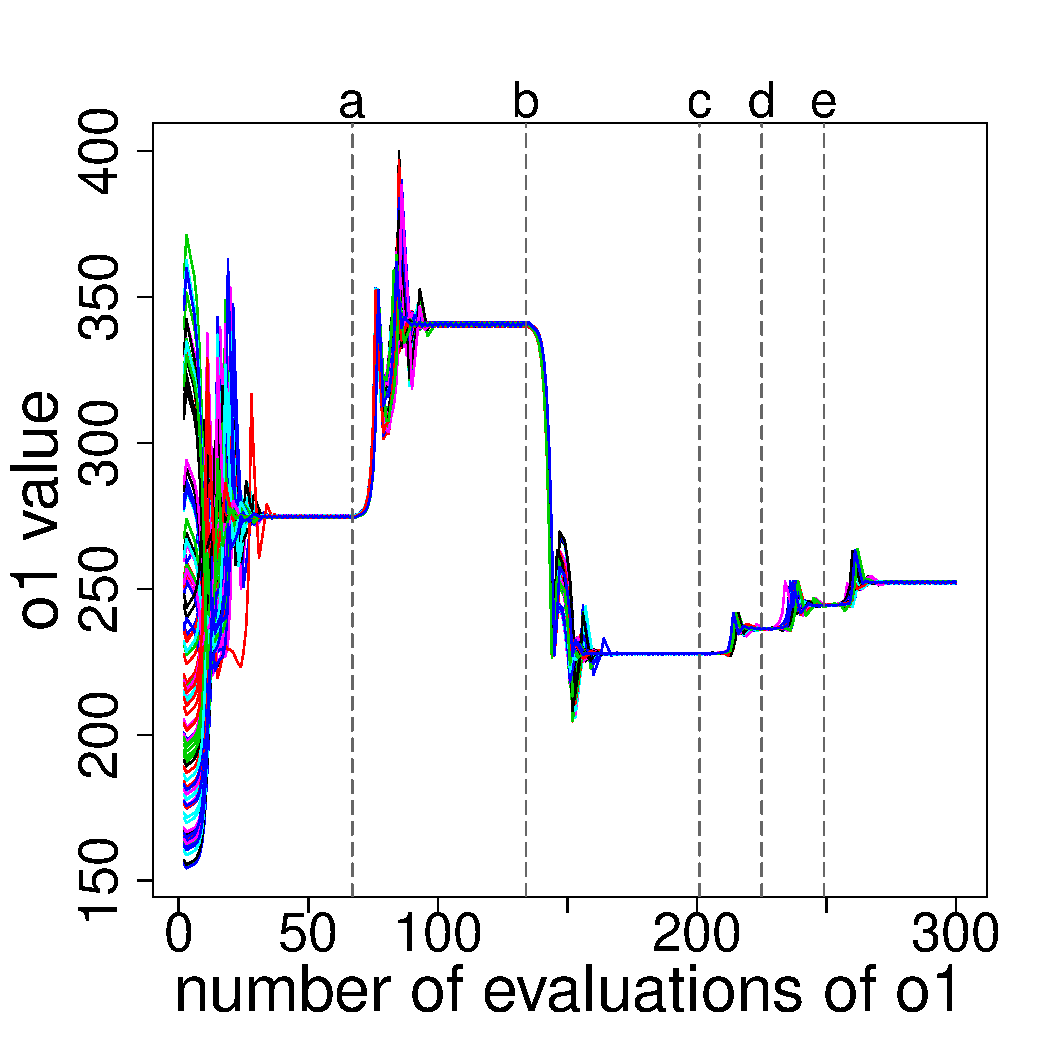
\includegraphics[width=\textwidth]{./R_figs/generated/turbofan_perturbated_o1}
		\label{turbofan_res_pert:o1}
	\end{minipage}}
	\subfloat{\begin{minipage}{0.32\textwidth}
		\centering
		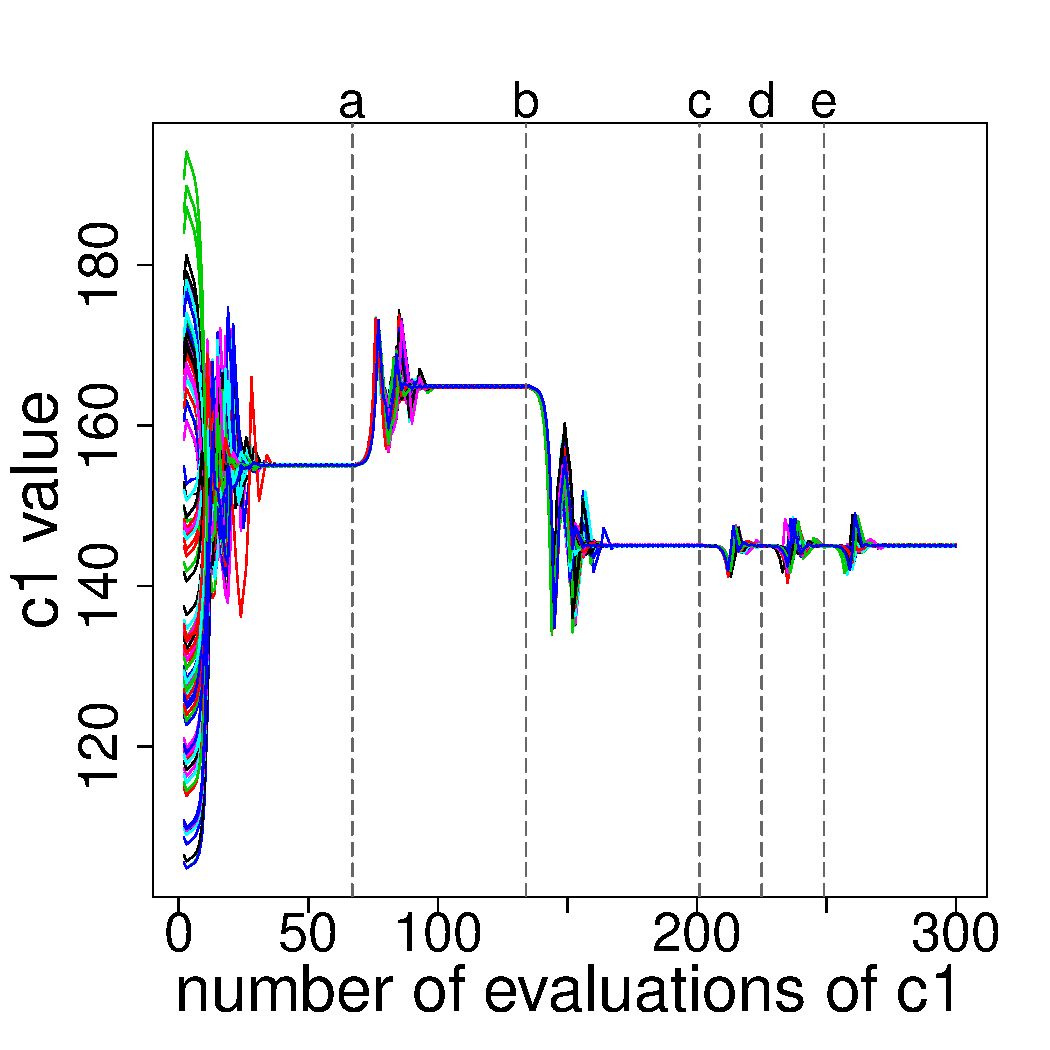
\includegraphics[width=\textwidth]{./R_figs/generated/turbofan_perturbated_c1}
		\label{turbofan_res_pert:c1}
	\end{minipage}}

	\subfloat{\begin{minipage}{0.32\textwidth}
		\centering
		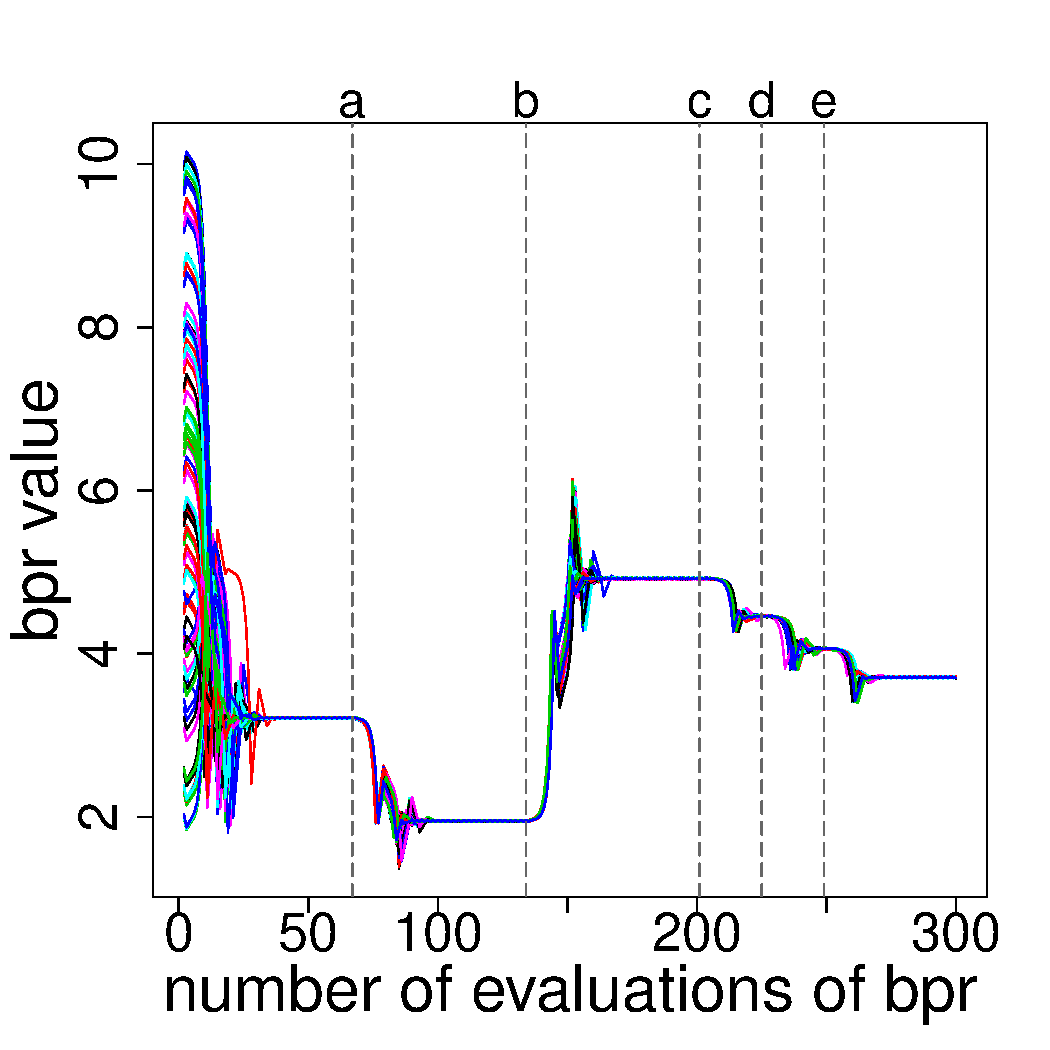
\includegraphics[width=\textwidth]{./R_figs/generated/turbofan_perturbated_bpr}
		\label{turbofan_res_pert:bpr}
	\end{minipage}}
	\subfloat{\begin{minipage}{0.32\textwidth}
		\centering
		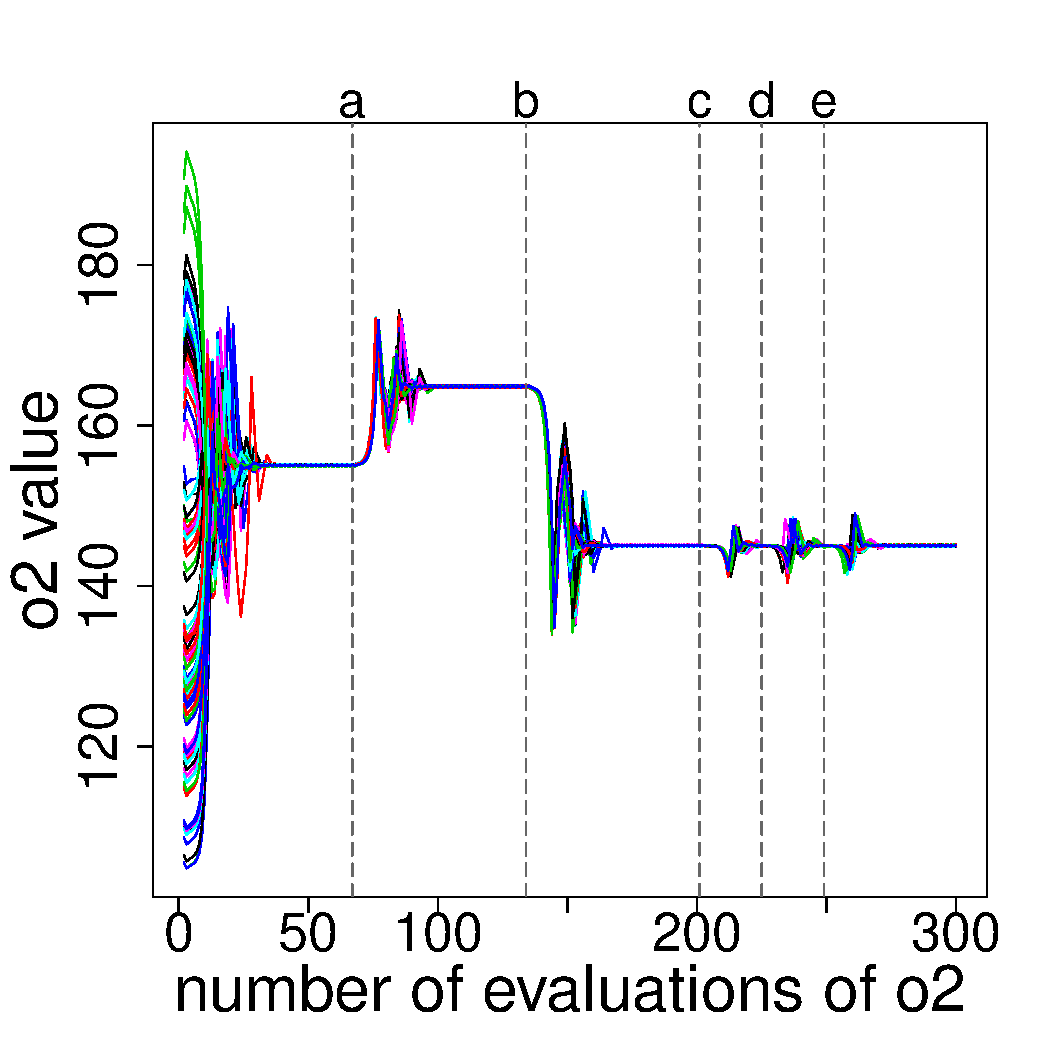
\includegraphics[width=\textwidth]{./R_figs/generated/turbofan_perturbated_o2}
		\label{turbofan_res_pert:o2}
	\end{minipage}}
	\subfloat{\begin{minipage}{0.32\textwidth}
		\centering
		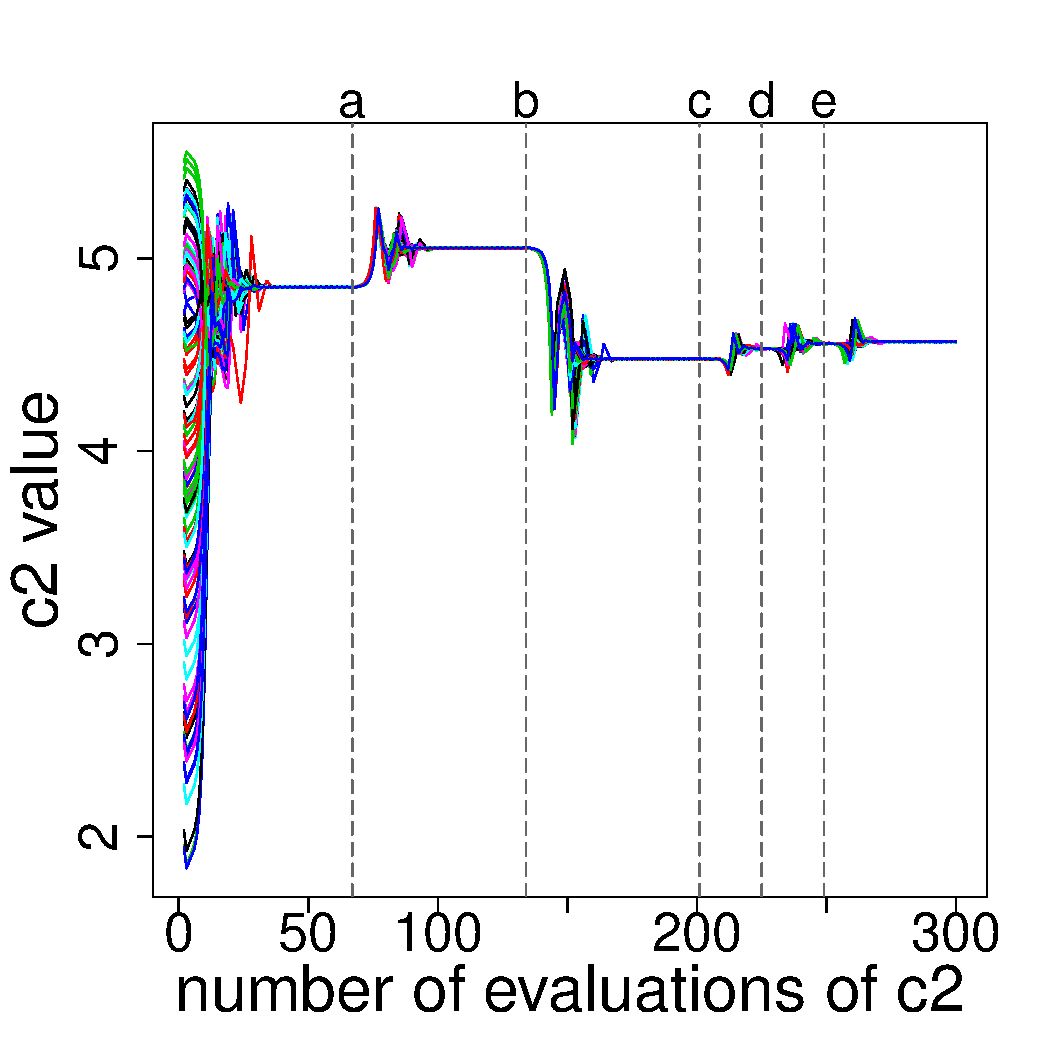
\includegraphics[width=\textwidth]{./R_figs/generated/turbofan_perturbated_c2}
		\label{turbofan_res_pert:c2}
	\end{minipage}}
	
	\caption{Turbofan agents behavior with perturbations (changes at dotted lines)}
	\label{turbofan_res_pert}
\end{figure*}


On \figurename{} \ref{turbofan_res_pert}, we illustrate the adaptation capabilities of the system by subjecting turbofan problem we introduced previously to a series of both strong and faster successive small changes to the problem topology (each perturbation is indicated  by a dotted line). \\
First we create strong changes by modifying simultaneously both a constraint and the definition domain of $pi\_c$:
\begin{description}
\item[a.] $c1$ changed from $s <= 155$ to $s <= 165$, max bound of $pi\_c$ changed from 40 to 50
\item[b.] $c1$ changed from $s <= 165$ to $s <= 145$, max bound of $pi\_c$ changed from 50 to 30
\end{description}
 Then milder perturbations by only changing the definition domain of the variable:
\begin{description}
\item[c.] max bound of $pi\_c$ changed from 30 to 35
\item[d.] max bound of $pi\_c$ changed from 35 to 40
\item[e.] max bound of $pi\_c$ changed from 40 to 45
\end{description}
The experiments show that the system consistently reacts to these perturbations by adapting itself in order to find a new solution for the modified problem.

\chapter{Large Tests Cases and Comparison with Existing Methods}

\section{Preliminary Aircraft Design}

\section{Snecma 2}

\section{Comparison with Existing Methods}

In this section we provide a comparison of our MAS with existing MDO methods. This comparison is based on the work of \cite{perez2004evaluation, Yi2008}. These two works are complementary as both of them concerns a common subset of representative MDO methods: MDF, IDF, CSSO, BLISS and CO.

The work of \cite{perez2004evaluation} presents an analysis of these methods based on two test cases and rank them on multiple criteria: \emmph{Accuracy, Efficiency, Transparency, Simplicity, Portability}.

The analysis of \cite{Yi2008} is based on different criteria, concentrating on the performances regarding the number of functions calls and the additional informations required by each methods. An interesting aspect of this comparison is that it provide several mathematical test cases on which the methods are applied.

For our evaluation we use the test cases provided by \cite{Yi2008} and compare the performances of the system to the existing MDO methods. We then provide a comparison synthesis based on the criteria and analysis presented in \cite{perez2004evaluation}.

In order to obtain comparable results with MDO methods, we adopted a problem modeling based on the disciplines dividing proposed in the works. To this end, we considered that, for every test cases, the natural formulation of the problem matched the discipline division proposed. Consequently, for each test case, the mathematical models represented by our models agents correspond to the proposed disciplines.

\subsection{Comparison Synthesis}
 
 Here we present a synthesis of the comparison between our system and existing MDO methods. For this comparison we use the criteria proposed in \cite{perez2004evaluation}, which are defined as follow:
 \begin{compactitem}
 \item \emph{Accuracy}: the quality of the solution proposed by the method, based on the distance between the solution and the real optimal values.
 \item \emph{Efficiency}: the computational cost to find the proposed solution, based on the number of disciplinary evaluations.
 \item \emph{Portability}: the feasibility to apply the method in the context of an existing work organization, based on the distributivity capabilities of the method.
 \item \emph{Simplicity}: the ease to instantiate and apply the method to different problems, based on the number of optimizers and variables required to implement the examples.
 \item \emph{Transparency}: the capability to understand, modify or extend the method.
 \end{compactitem}
 
 \paragraph*{}
 The \emph{Accuracy} criterion [[TODO]]
 
 \paragraph*{}
 The \emph{Efficiency} criterion [[TODO]]
When counting the number of evaluation calls, a distinction is made between discipline evaluations and full problem evaluations, the latter being considered considerably more costly than the former.

Our MAS does not require any full problem evaluation, using only disciplines evaluations.
 
 \paragraph*{}
 The \emph{Portability} criterion concerns the feasibility to integrate the method into an existing organizational structure. This evaluation criterion is based on the capabilities of the method to divide the concerns to match existing expert teams or specializations. In this regard, our method is extremely portable as it support multiple levels of modeling and multiple reformulations of the problem. Consequently the problem can be \enquote{tailored} to fit the existing organizational structure. Contrary to the MDO methods, our method does not mandate a \emph{central} authority as the responsibility to maintaining consistency is distributed in the system.
  
 \paragraph*{}
  The \emph{Simplicity} criterion concerns the amount of work required to instantiate the method to suit different optimization problem. The original authors chose to evaluate this criterion using to measures: the number of optimizers involved and the number of additional variable required by the method. Regarding the number of objectives, our method requires $n$ optimizers ($n$ being the number of models involved). In this regard it is less efficient than MDF and IDF, which only require 1 optimizer, but is better than the other methods which require $n+1$ optimizers (1 by model plus 1 global optimizer). In regard of the number of additional variables, our method in on part with MDF, the best method in regard of this measure, as neither of them require any additional variable.
Consequently, the only method dominating our own in regard of this criterion is MDF. Our method can be considered on part with IDF, as neither of them dominate the other on both measures.  
  
 \paragraph*{}
 The \emph{Transparency} criterion is the less well-defined and the can be perceived as somewhat subjective. The original authors give as an example \enquote{a probability-based method can be seamlessly integrated into a transparent formulation, which does not require major changes of the architecture to accomplish the integration.} In this regard we have shown that our approach was modular and extensible, due to the distribution of roles between the agents and to the explicity encapsulation of mathematical tools (analytical models, external optimizers). We demonstrated this modularity with the addition of uncertainty propagation mechanisms into the MAS.
 
 \paragraph*{}

\begin{table}
\caption{Classification by criteria (based on \cite{perez2004evaluation})}
\centering
\begin{tabular}{cccccc}
		\toprule
			& Accuracy & Efficiency & Transparency & Simplicity & Portability\\
		\midrule
		b\tn{a1}est& \textbf{AMAS} & \textbf{AMAS} & \textbf{AMAS} & MDF & \textbf{AMAS}\\
			& MDF & IDF & MDF & IDF, \textbf{AMAS} & CO\\
			& IDF & BLISS & IDF &  & CSSO\\
			& BLISS & CSSO & CO & CO & BLISS\\
			& CO & CO & CSSO & CSSO & IDF\\
		wo\tn{a2}rst& CSSO & MDF & BLISS & BLISS & MDF\\
		\bottorule
\end{tabular}
\tikz[remember picture,overlay]
    \path[->, very thick] (a1.south) edge (a2.north -| a1.south);
\end{table}

\chapter{Evaluating Performances using Generated Test Cases and Scalability}

In this section we present some measures we established in regard of the scalability performances of our MAS. [[TOCHANGE if spring networks are integrated]] For this part of the experiments we were not concerned with the optimization performances of the system, but more with its capability to handle large agent graphs without suffering from performances degradation.

\section{Generating NDMO Agent Graphs}

In order to realize our experiments, we required a large number of test cases of several sizes and comparable complexity.  Since such repository of continuous optimization problems is not readily available, we worked on a way to automatically generate them. To this end, we took advantage of the fact that, as demonstrated with our NDMO modeling, an optimization problem can be represented as a graph. Consequently it is possible to use well-known graph generation techniques and directly generate problem graphs.

We propose a very simple method to generate simple problem graphs. First we use a graph generation algorithm to generate a directed graph of size $n$. The nodes of this graph represent the variables of the problem and the arcs their dependencies. If a node is not the head of any arc (\emph{i.e.} there is no arc going to this node), it is a design variable, otherwise it is an output variable.\\
The next step is to insert models. As we stated, the optimization problem in itself is of little importance in this part. Consequently our only requirement for the model is that they must be able to take an arbitrary number of inputs and produce one output. In our experiments we used a simple \emph{Sum} function. For each output variable, we insert a node representing the model in the graph. The links going to the output variable node are redirected to the model node, and a link going from the model node to the output node is create.\\
After this step, criteria are randomly added to variable nodes. In our experiments, we given a 20\% probability of a variable node  to be linked to a criterion, with half the chance for the criterion to be an objective and half the change for it to be a constraint. Once more, in order to simplify the problem generation, all objectives are about minimizing the variable, and are constraints are about having the variable higher of equal to zero.

The generation method is summarized in \ref{algo_graph_generation}. After all these steps, the graph is a valid [[(if not useful)]] NDMO graph and can be directly transformed into an agent graph.

\begin{algorithm}
\caption{Problem graph generation}
\label{algo_graph_generation}
	$n \leftarrow$ initialization number
	$G(nodes, arcs) \leftarrow GraphGenerator(n)$\;
			
		\ForEach{$currentNode \in G.nodes$}{
			tag($currentNode$, \enquote{variable})\;
			$enteringArcs \leftarrow \{arc \in G.arcs, isHeadOf(arc, currentNode)\}$
			\If{$enteringArcs \neq \emptyset$}{
				\tcp{$currentNode$ is an output variable}
				$modelNode \leftarrow $ new node\;
				tag($modelNode$, \enquote{model})\;
				$G$.add($modelNode$)\;
				$G$.createArcBetween($modelNode$, $currentNode$)\;
				\ForEach{$arc \leftarrow enteringArcs$}{
					$tailNode \leftarrow arc.tail$\;
					$G$.removeArc($arc$)\;
					$G$.createArcBetween($tailNode$, $modelNode$)\;
				}
			}
			\;
			\tcp{check for criteria}			
			$rand \leftarrow drawRandomNumber()$\;		
			\If{$rand \leq	 criteriaProba$}{		
				$critNode \leftarrow$ new node\;
				$G$.createArcBetween($currentNode$, $critNode$)\;
				\eIf{$rand \leq drawRandomNumber/2$}{
					tag($critNode$, \enquote{objective})\;				
				}{
					tag($critNode$, \enquote{constraint})\;
				}
			}		
		}

\end{algorithm}

It must be noted that the final size of problems generated by this algorithm is not fixed, and can be significantly larger than the initialization value $n$. However problems produced using the same initialization number and the same graph generator are of comparable sizes.

We used graph generators proposed by the GraphStream library \footnote{\url{http://www.graphstream-project.org/}}. On \figurename{} \ref{graph_generation_examples} some examples of graphs produced using these generators are visualized using GraphStream visualization tools. It should be noted that, because  of the modifications we apply on the graph after it is created using the generator, the final agent graph does not necessarily respect the properties of the initial graph , however we can see on \figurename{} \ref{graph_generation_examples} that, the modifications we apply do not radically modify the characteristic topologies of the different graph types.
 
\begin{figure}
\centering
	\begin{subfigure}[b]{0.45\textwidth}
		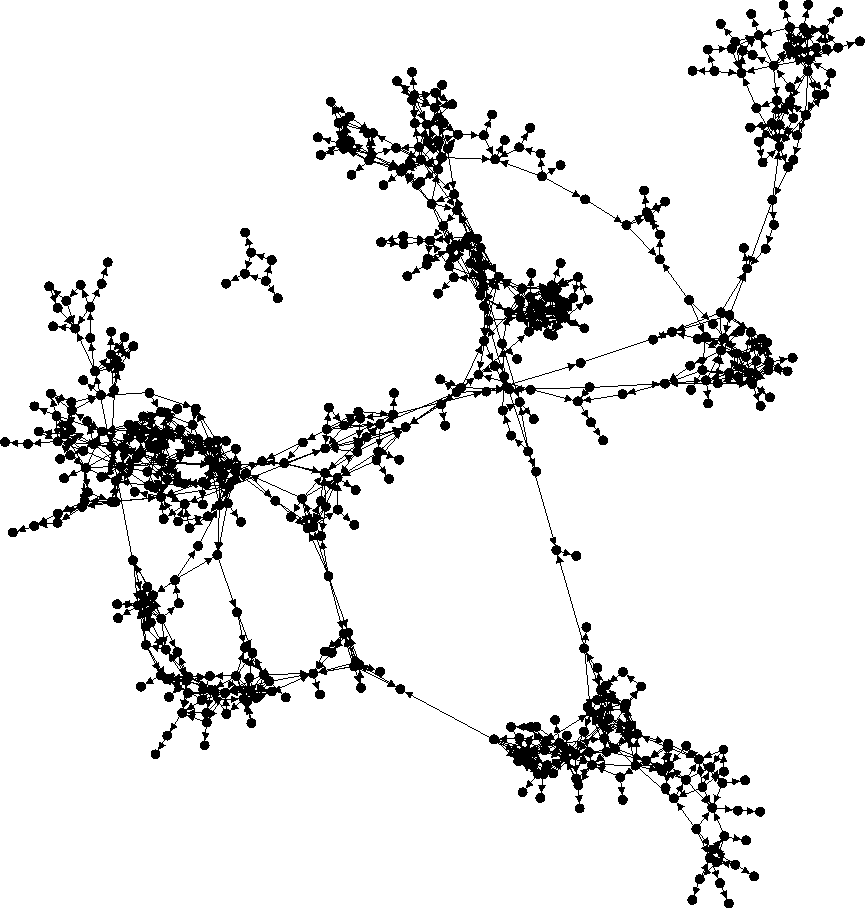
\includegraphics[width=\textwidth]{graph_random_euclid_1}
		\caption{Random Euclidean graph example 1.}\label{generatedgraphs:rand1}
	\end{subfigure}
	\begin{subfigure}[b]{0.45\textwidth}
			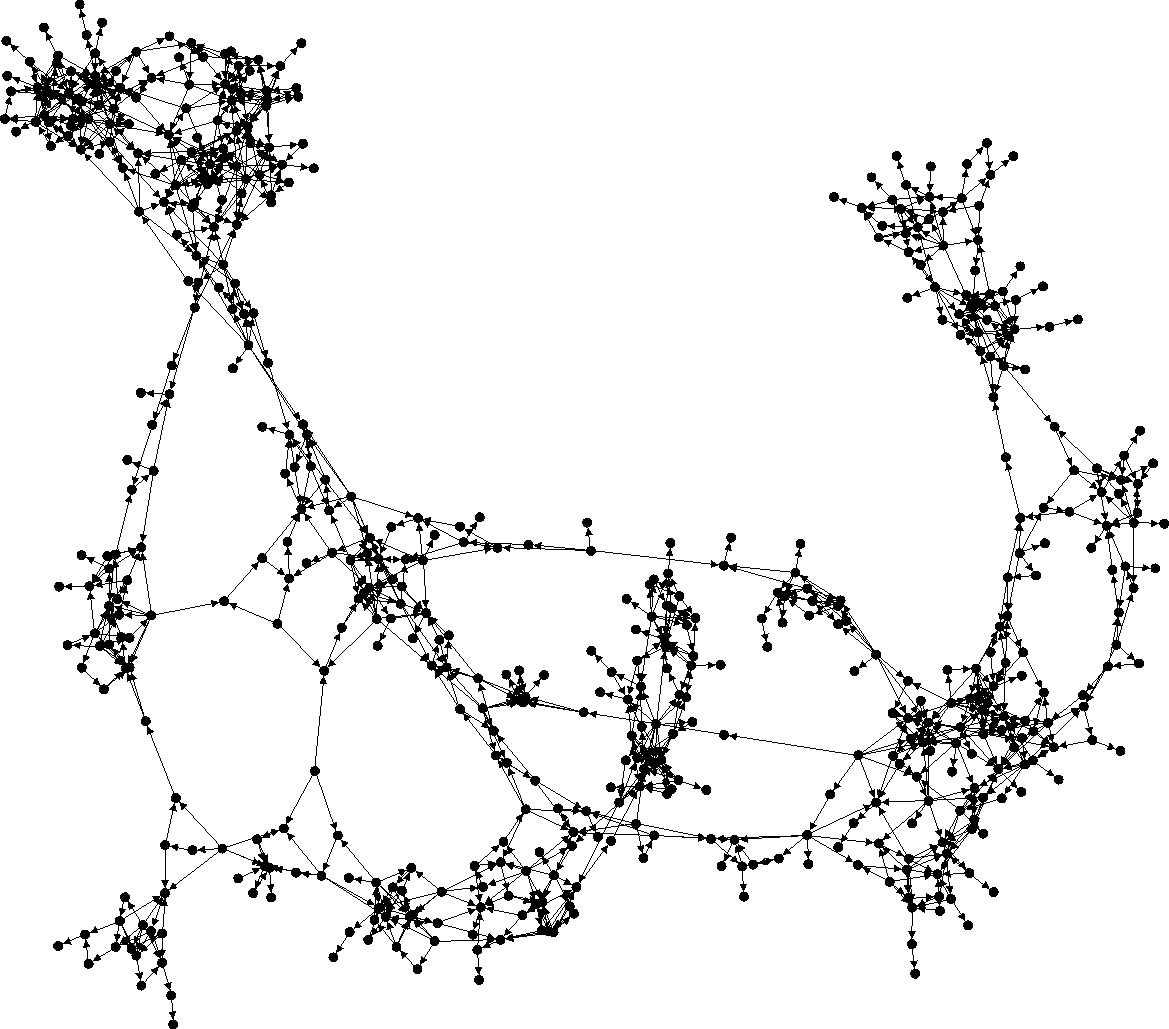
\includegraphics[width=\textwidth]{graph_random_euclid_2}
		\caption{Random Euclidean graph example 2.}\label{generatedgraphs:rand2}
	\end{subfigure}
	
	\begin{subfigure}[b]{0.45\textwidth}
		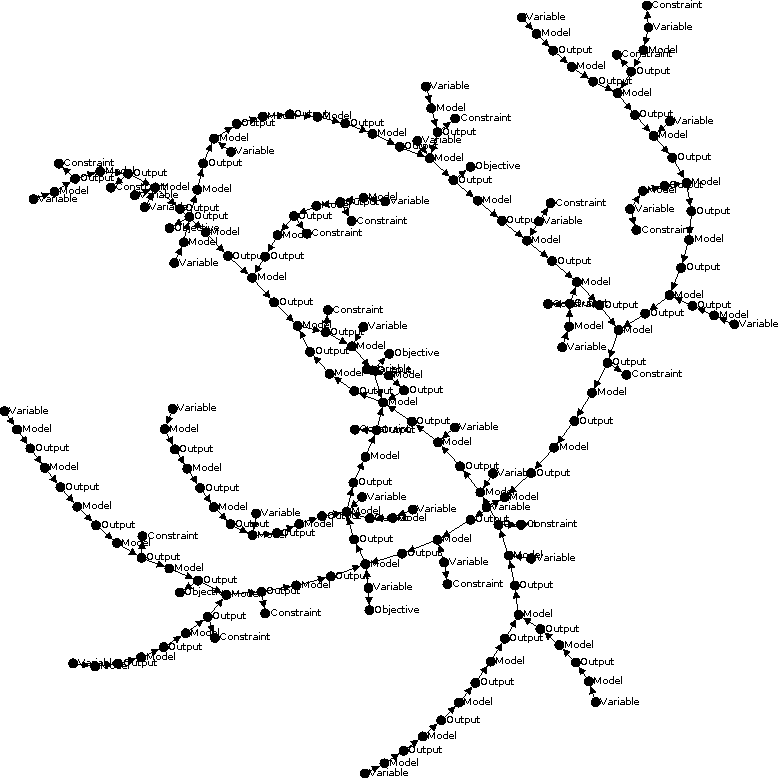
\includegraphics[width=\textwidth]{graph_SW_1}
		\caption{Small-World graph example 1.}\label{generatedgraphs:sw1}
	\end{subfigure}
	\begin{subfigure}[b]{0.45\textwidth}
			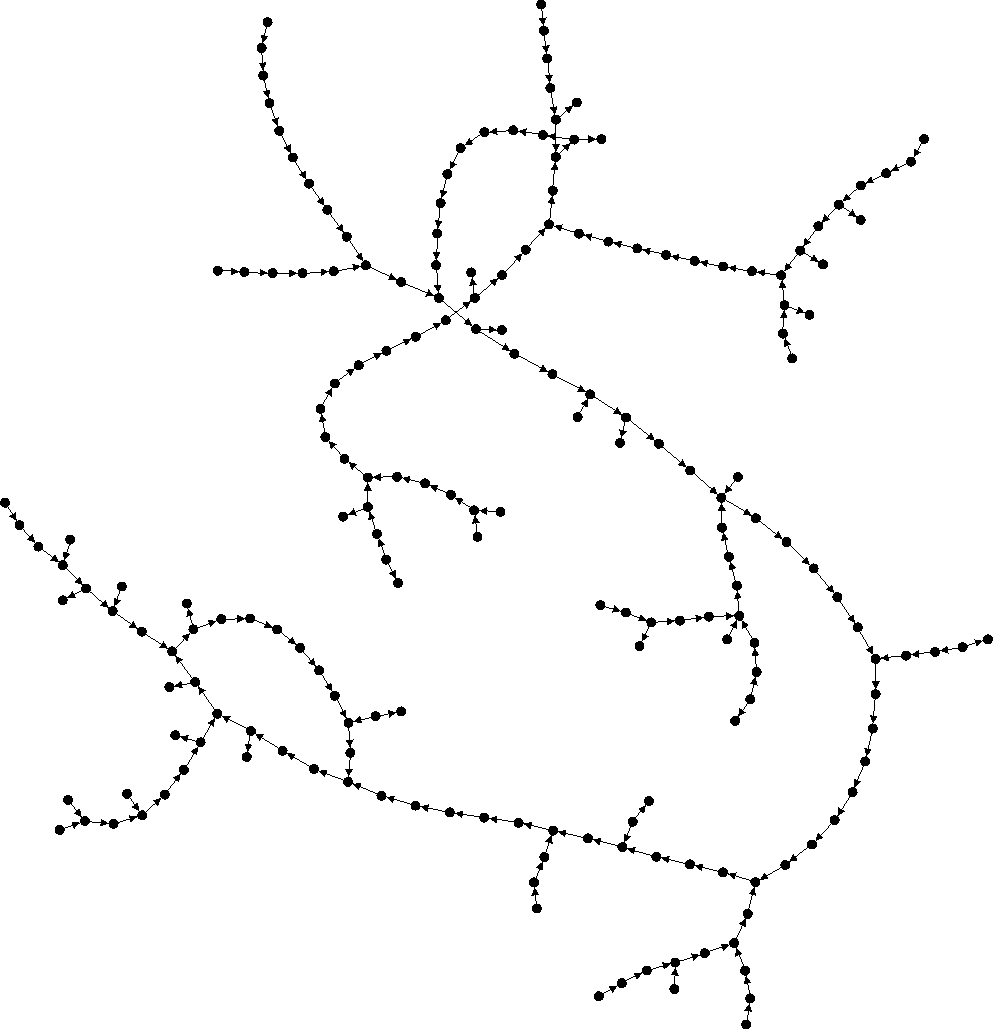
\includegraphics[width=\textwidth]{graph_SW_2}
		\caption{Small-World graph example 2.}\label{generatedgraphs:sw2}
	\end{subfigure}

\caption{Examples of graph generation.}
\label{graph_generation_examples}
\end{figure}

\section{Experimental Results}

Before discussing the results we obtained, let us add a word of warning concerning measuring real-time performances of java applications (java being the programming language used to implement our prototype). The Java Virtual Machine (JVM), which executes java programs, applies a lot of complex optimization steps \emph{during} the execution process. Consequently making some precise and non-biased measurements can be hazardous.\\
Regarding our experiments, we tried to mitigate possible bias by taking the two following precautions:
\begin{compactitem}
\item before running the measured experiments, running multiple problems whose results were discarded, in order to \enquote{heat} the JVM and allowing it to apply its optimization procedures beforehand.
\item running the different experiments multiple times and in different orders, to \enquote{spread} the benefits of possible optimizations happening at runtime.
\end{compactitem}
We believe that these precautions are sufficient to obtain sufficiently meaningful results. Nevertheless, the reader should be warned not to consider the presented values as exact measurements of the system performances.

On \figurename{} \ref{time_by_size_perfo} are presented the results of the execution time of problems of different sizes. We generated agent graphs of different sizes using both Small-Word and Random Euclidean algorithms. On the figure are presented the mean time needed for all the agents of the problem to execute 800 behavior cycle. Interestingly, while the time performances in regard of small-world based problems graphs increase linearly with the size of the problems, the time needed in the case of random problem graphs seems to increase exponentially.

\begin{figure}
\centering

	\begin{subfigure}[b]{0.45\textwidth}
		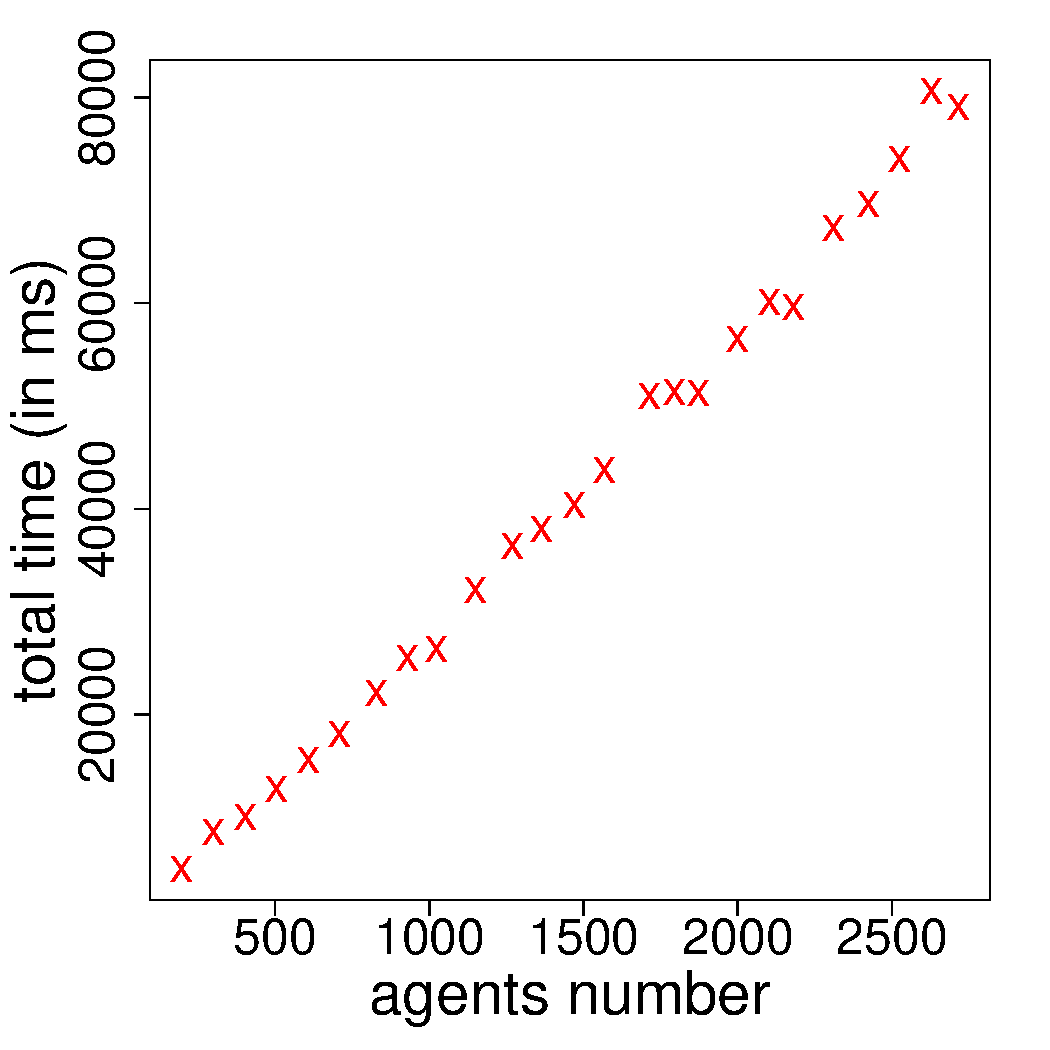
\includegraphics[width=\textwidth]{R_figs/graph_problems/time_by_size_watts_strogatz}
		\caption{Small-World graphs.}\label{time_by_size_perfo:ws}
	\end{subfigure}
	\begin{subfigure}[b]{0.45\textwidth}
			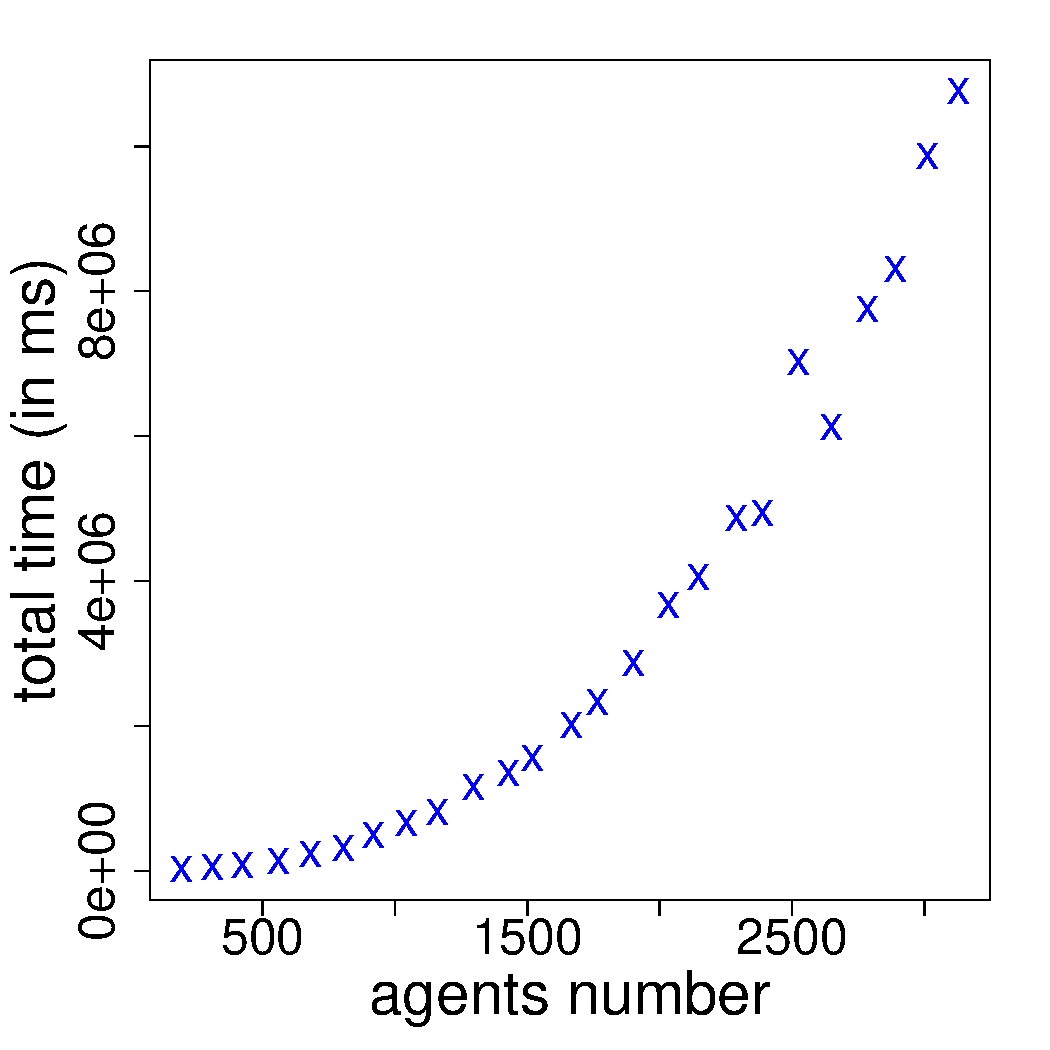
\includegraphics[width=\textwidth]{R_figs/graph_problems/time_by_size_random_eclidean}
		\caption{Random Euclidean graphs.}\label{time_by_size_perfo:re}
	\end{subfigure}

\caption{Time performances by MAS size.}\label{time_by_size_perfo}
\end{figure}

This seemingly poor performance can however easily be explained by looking at \figurename{} \ref{degree_by_size}, on which are shown the mean degree (that is, the number of arcs entering of exiting a node) of the nodes in each generated problems. We can see, that, whatever the size of the problem, the mean degree of a node in Small-World problems is mostly constant. However, in the case of Random Euclidean graphs, the mean degree increases linearly with the size of the problem. Consequently, the exponential increase in time regarding Random Euclidean graphs can be explained by the conjugated effects of the increase in number of agents and the increase of the neighborhood size of the agents (whose impact in the behavior algorithm complexity has been exposed in section \ref{NCS_pres}).

\begin{figure}
\centering
			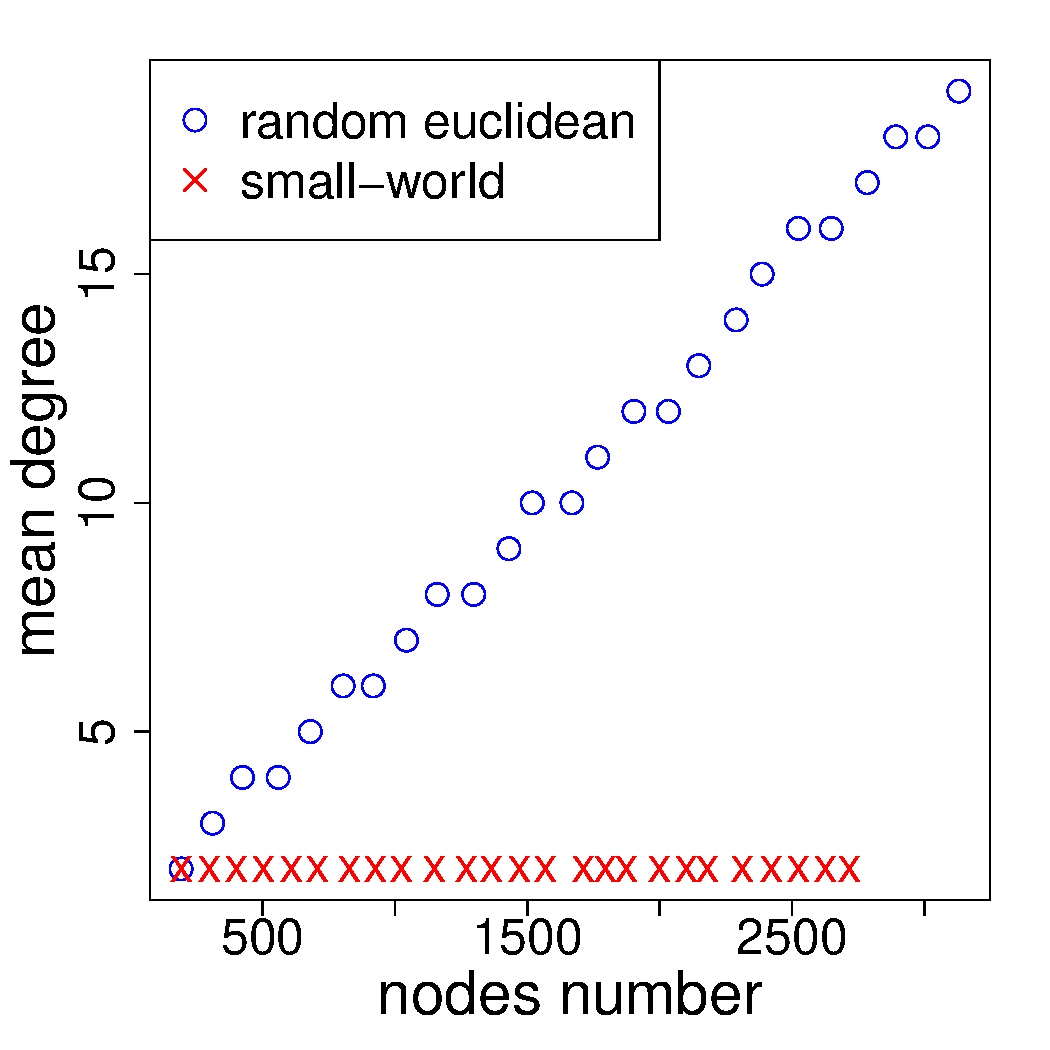
\includegraphics[width=0.45\textwidth]{R_figs/graph_problems/degree_by_size_comparison}
\caption{Comparison of nodes mean degree by graph type.}\label{degree_by_size}
\end{figure}

In order to corroborate this analysis, we studied the impact increasing the nodes degree has on the execution time of the MAS. On \figurename{} \ref{experiment_degrees}, we show the results of another experiment using agent graphs generated using a Barabasi-Albert generator, which has the advantage of being able to easily generate graphs with different mean degree sizes at the cost of only a slight increase of node numbers. On the figure is shown the average time for all the agents to make a behavior cycle in function of the mean degree of the agents (using Barabasi-Albert based graphs of sizes between 510 and 550 nodes). We can see that the neighborhood size of the agents (the degree of the node) has the predicted effect on the time needed by the agents to execute their behavior.

\begin{figure}
\centering
	\begin{subfigure}[b]{0.45\textwidth}
		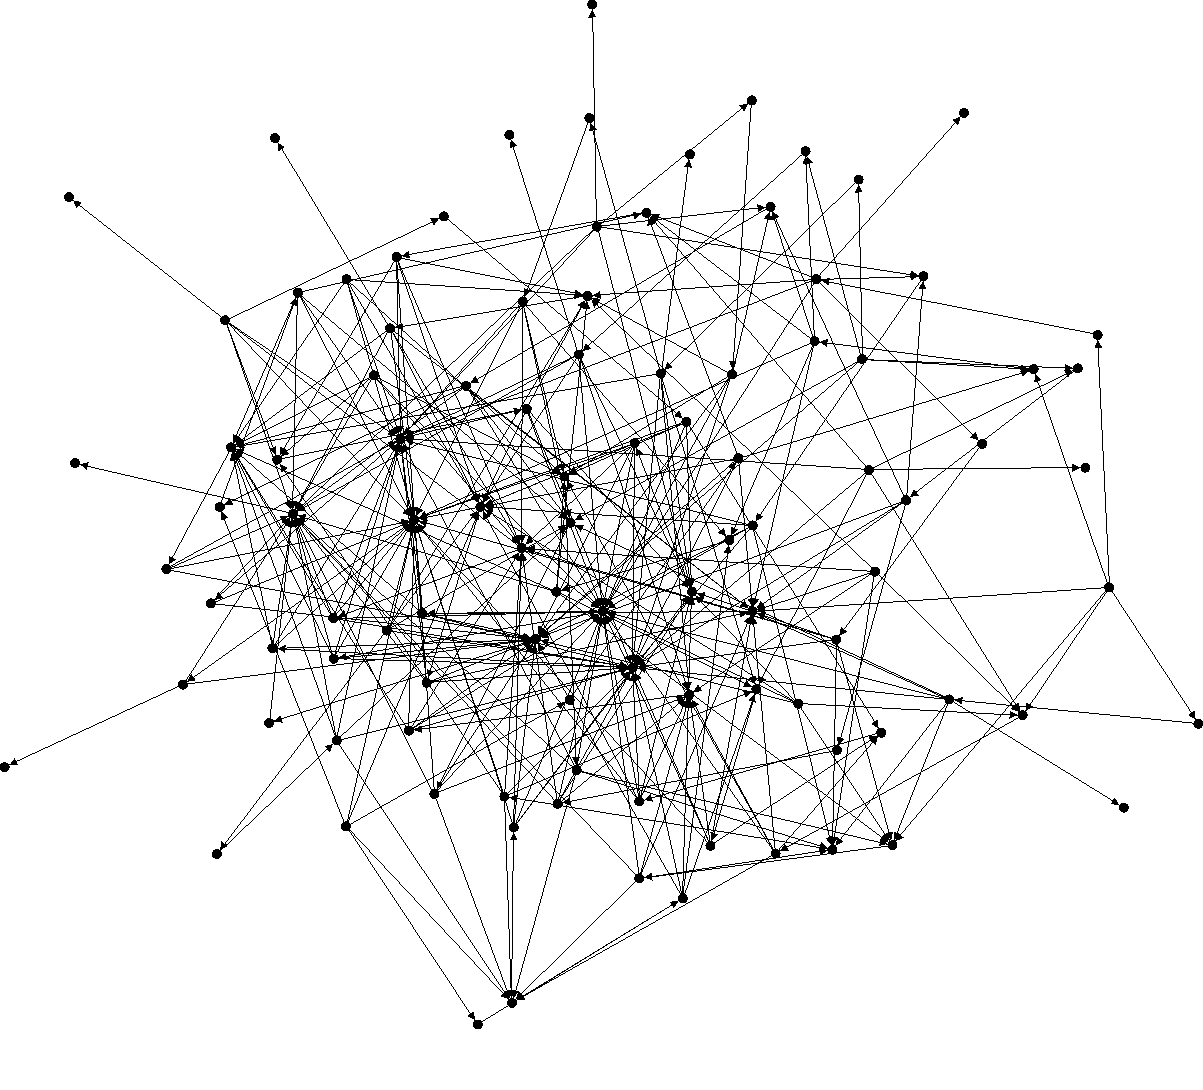
\includegraphics[width=\textwidth]{graph_barabasi_albert}
		\caption{Barabasi-Albert graph example.}\label{experiment_degrees:graph}
	\end{subfigure}
	\begin{subfigure}[b]{0.45\textwidth}
			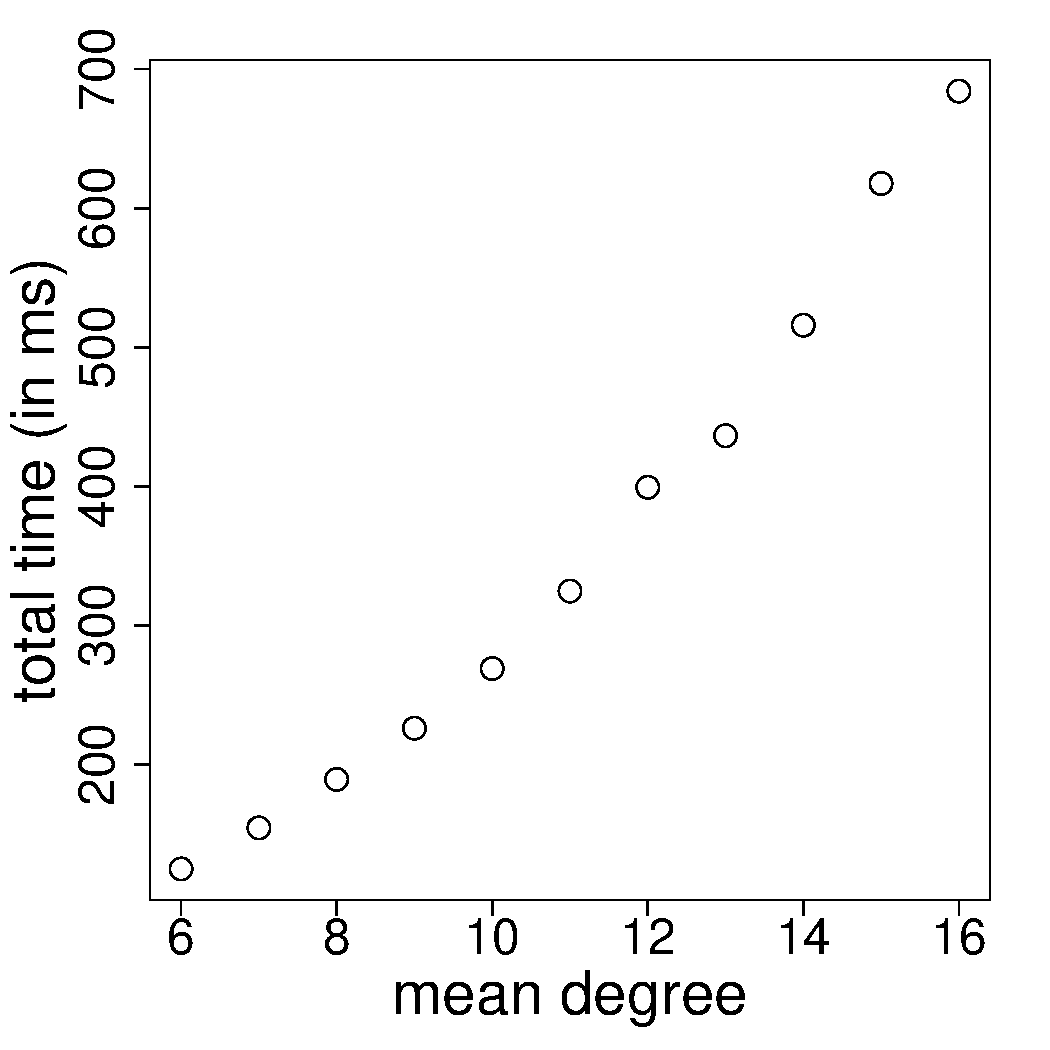
\includegraphics[width=\textwidth]{R_figs/graph_problems/time_by_degree_barabasi_albert}
		\caption{Average time for a step (by mean degree).}\label{experiment_degrees:res}
	\end{subfigure}
\caption{Time performances by node degree.}
\label{experiment_degrees}
\end{figure}

\section{Analysis of Performances}

Overall, we can conclude by observing these results that the time required for the agents to make a behavior cycle is not meaningfully impacted by the size of the problem. This property is an expected benefit of restricting the agents to local perception and decision process.\\
The results also shown the impact of increasing the neighborhood size of the agents. The time increase correspond to the analysis we made concerning the computational complexity of the agent behavior (in \ref{NCS_pres}).  This analysis illustrates once more the importance of maintaining the behavior of the agents at a local level. Had the agent decision process involved not only its immediate neighbors, but also a large group of agent, the computational cost would have increased even more sharply with the size of the problem.\\
As a remark, let us add that our implementation of the agent behavior was far from optimal from a performances point of view. In order to modify and experiment more easily on the agents, we voluntary kept separated into distinct modules the different solving mechanism of the agents. A more efficient implementation could factor several of the treatments in order to reduce the computational complexity, obtaining a non-negligible performances improvement in the process.